\pagestyle{fancy}
\thispagestyle{fancy}
\chapter{Prototyping}
\section{Introduction to Prototyping}

For the prototyping phase to be successful, we must employ multiple techniques to enable users to assess the product idea in multiple situations and provide their input. While developing prototypes for a health data management platform, we must keep in mind the user interface, data visualization, and interaction patterns. Some common techniques used for implementing the prototype phases are:

\subsection{List of options available for Prototyping}

\begin{enumerate}
    \item \textbf{Wireframes and Sketches}\\
    Initial low-fidelity designs to illustrate the layout and structure of key interfaces. These help team members visualize the user flow and information hierarchy without getting caught up in visual design details.

    \item \textbf{Figma Prototypes}\\
    Creating interactive interfaces in Figma helps visualize the user experience and test navigation flows. These medium-fidelity prototypes allow for quick iterations and user feedback.

    \item \textbf{Interactive Components}\\
    Development of key UI components using Next.js and Tailwind CSS to test real functionality and interactions. This helps validate technical feasibility and user experience.

    \item \textbf{Data Visualization Mockups}\\
    Creating sample visualizations using tools like Recharts to prototype how health data will be displayed and interacted with.

    \item \textbf{API Integration Prototypes}\\
    Building functional prototypes to test integration with health data sources, sensors, and AI services. This validates technical feasibility and data flow.

    \item \textbf{Responsive Design Prototypes}\\
    Testing the application's responsiveness across different devices and screen sizes to ensure consistent user experience.

    \item \textbf{Animation Prototypes}\\
    Creating motion design prototypes using Framer Motion to test micro-interactions and transitions that enhance user experience.
\end{enumerate}

\subsection{Prototype Selected}
For our final implementation, we chose to combine several prototyping approaches:

\begin{itemize}
    \item High-fidelity Figma designs for user interface
    \item Next.js components for functional implementation
    \item Tailwind CSS for responsive styling
    \item Framer Motion for animations
    \item Supabase for database
\end{itemize}

\begin{figure}[H]
    \centering
    \includegraphics[width=0.8\textwidth]{figures/tech_stack.png}
    \caption{Technology Stack Overview}
\end{figure}

\section{Prototyping Implementation}
\subsection{Software Architecture}

\begin{figure}[H]
    \centering
    \includegraphics[width=1.0\textwidth]{figures/software_architecture.png}
    \caption{System Architecture Diagram}
\end{figure}

\subsubsection{Architecture Components}
Our system architecture leverages modern technologies for each layer:

\begin{itemize}
    \item \textbf{Frontend Layer}
    \begin{itemize}
        \item Next.js 14 for server-side rendering and routing
        \item React with TypeScript for type-safe development
        \item Tailwind CSS for responsive styling
        \item Framer Motion for smooth animations
    \end{itemize}

    \item \textbf{Backend Services}
    \begin{itemize}
        \item FastAPI for high-performance Python backend
        \item Real-time data processing and analytics
        \item Integration with AI/ML services
    \end{itemize}

    \item \textbf{Database Layer}
    \begin{itemize}
        \item Supabase Vector Database for semantic search
        \item Supabase SQL Database for structured data
        \item Real-time subscriptions for live updates
    \end{itemize}

    \item \textbf{AI/ML Integration}
    \begin{itemize}
        \item LangChain for RAG pipeline implementation
        \item OpenAI for text processing and generation
        \item Google Gemini Pro for multimodal analysis
    \end{itemize}

    \item \textbf{IoT Integration}
    \begin{itemize}
        \item Arduino sensors for health data collection
        \item Real-time data streaming and processing
        \item Secure data transmission protocols
    \end{itemize}
\end{itemize}

\subsection{Core Components}

\subsubsection{RAG Pipeline Architecture}
\begin{figure}[H]
    \centering
    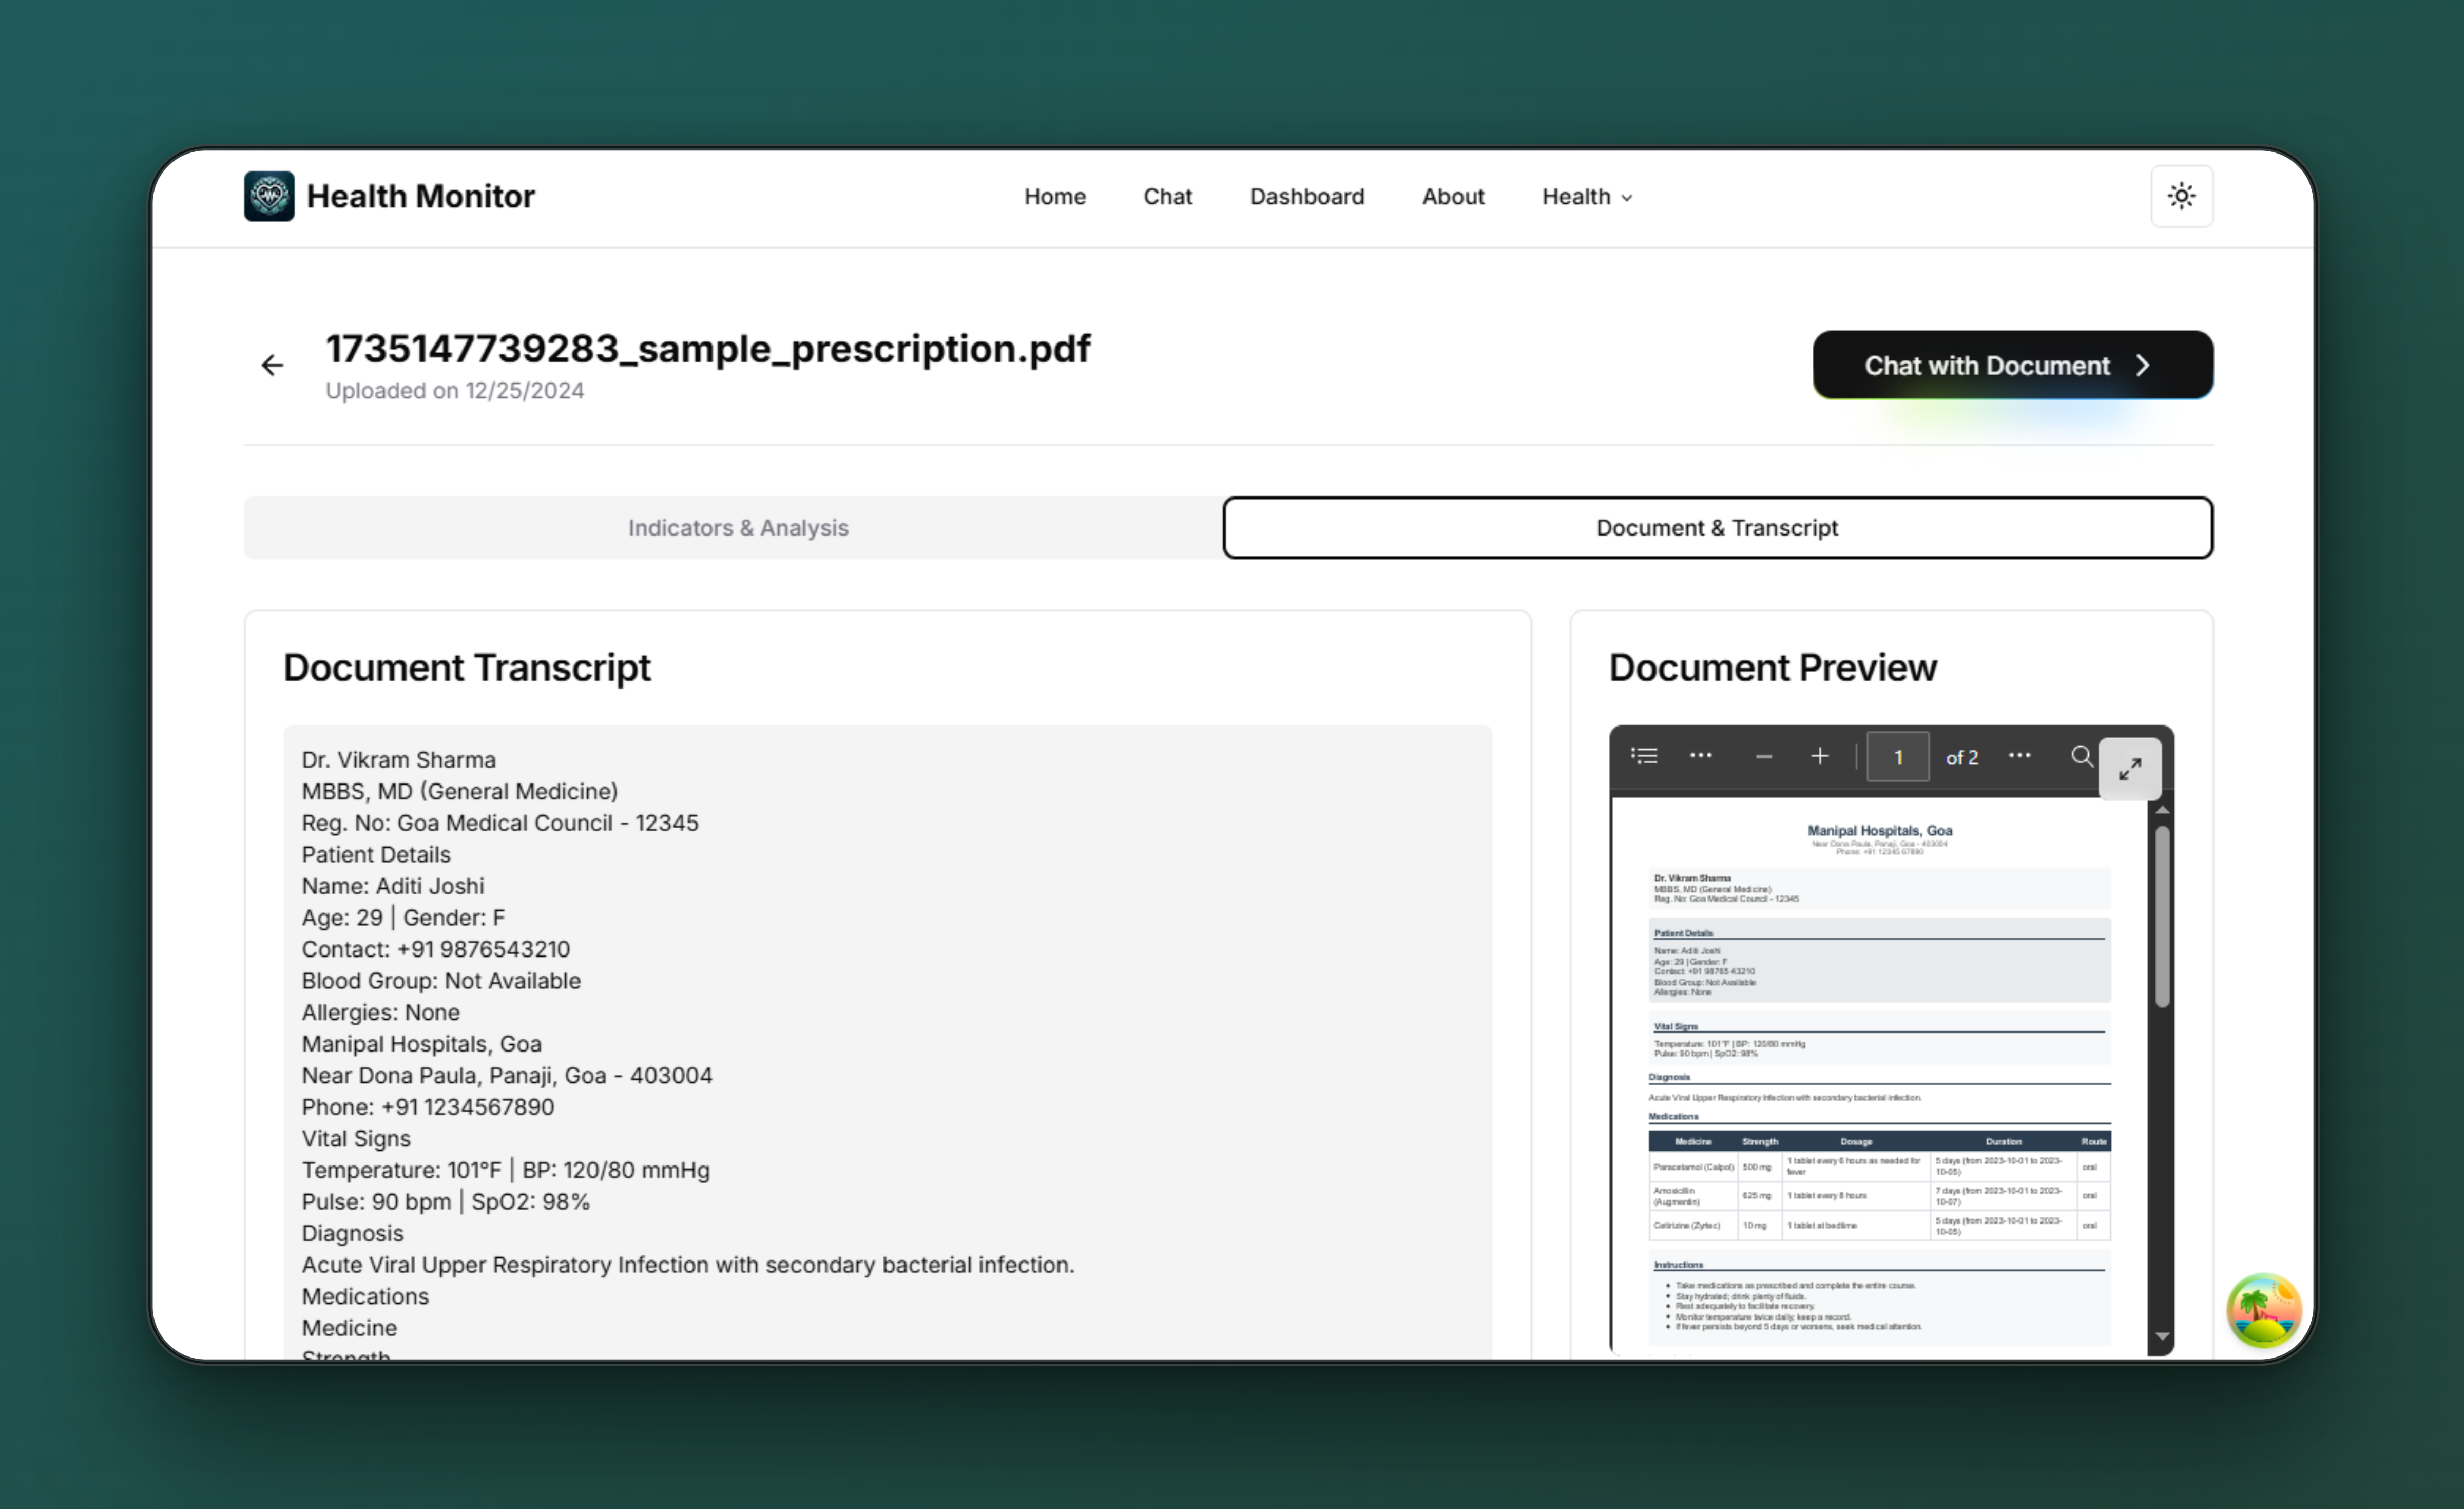
\includegraphics[width=0.8\textwidth]{public/landing/hm-record-transcript.png}
    \caption{Document Processing and Analysis Pipeline}
\end{figure}

Key components of the RAG pipeline:
\begin{enumerate}
    \item \textbf{Data Ingestion}
    \begin{itemize}
        \item Document processing (PDF, images)
        \item Sensor data integration
        \item Medical record parsing
    \end{itemize}

    \item \textbf{Data Processing}
    \begin{itemize}
        \item Text extraction and OCR
        \item Embedding generation
        \item Vector database storage
    \end{itemize}

    \item \textbf{Information Retrieval}
    \begin{itemize}
        \item Semantic search
        \item Context-aware querying
        \item Real-time data aggregation
    \end{itemize}
\end{enumerate}

\subsection{AI Integration}
\begin{figure}[H]
    \centering
    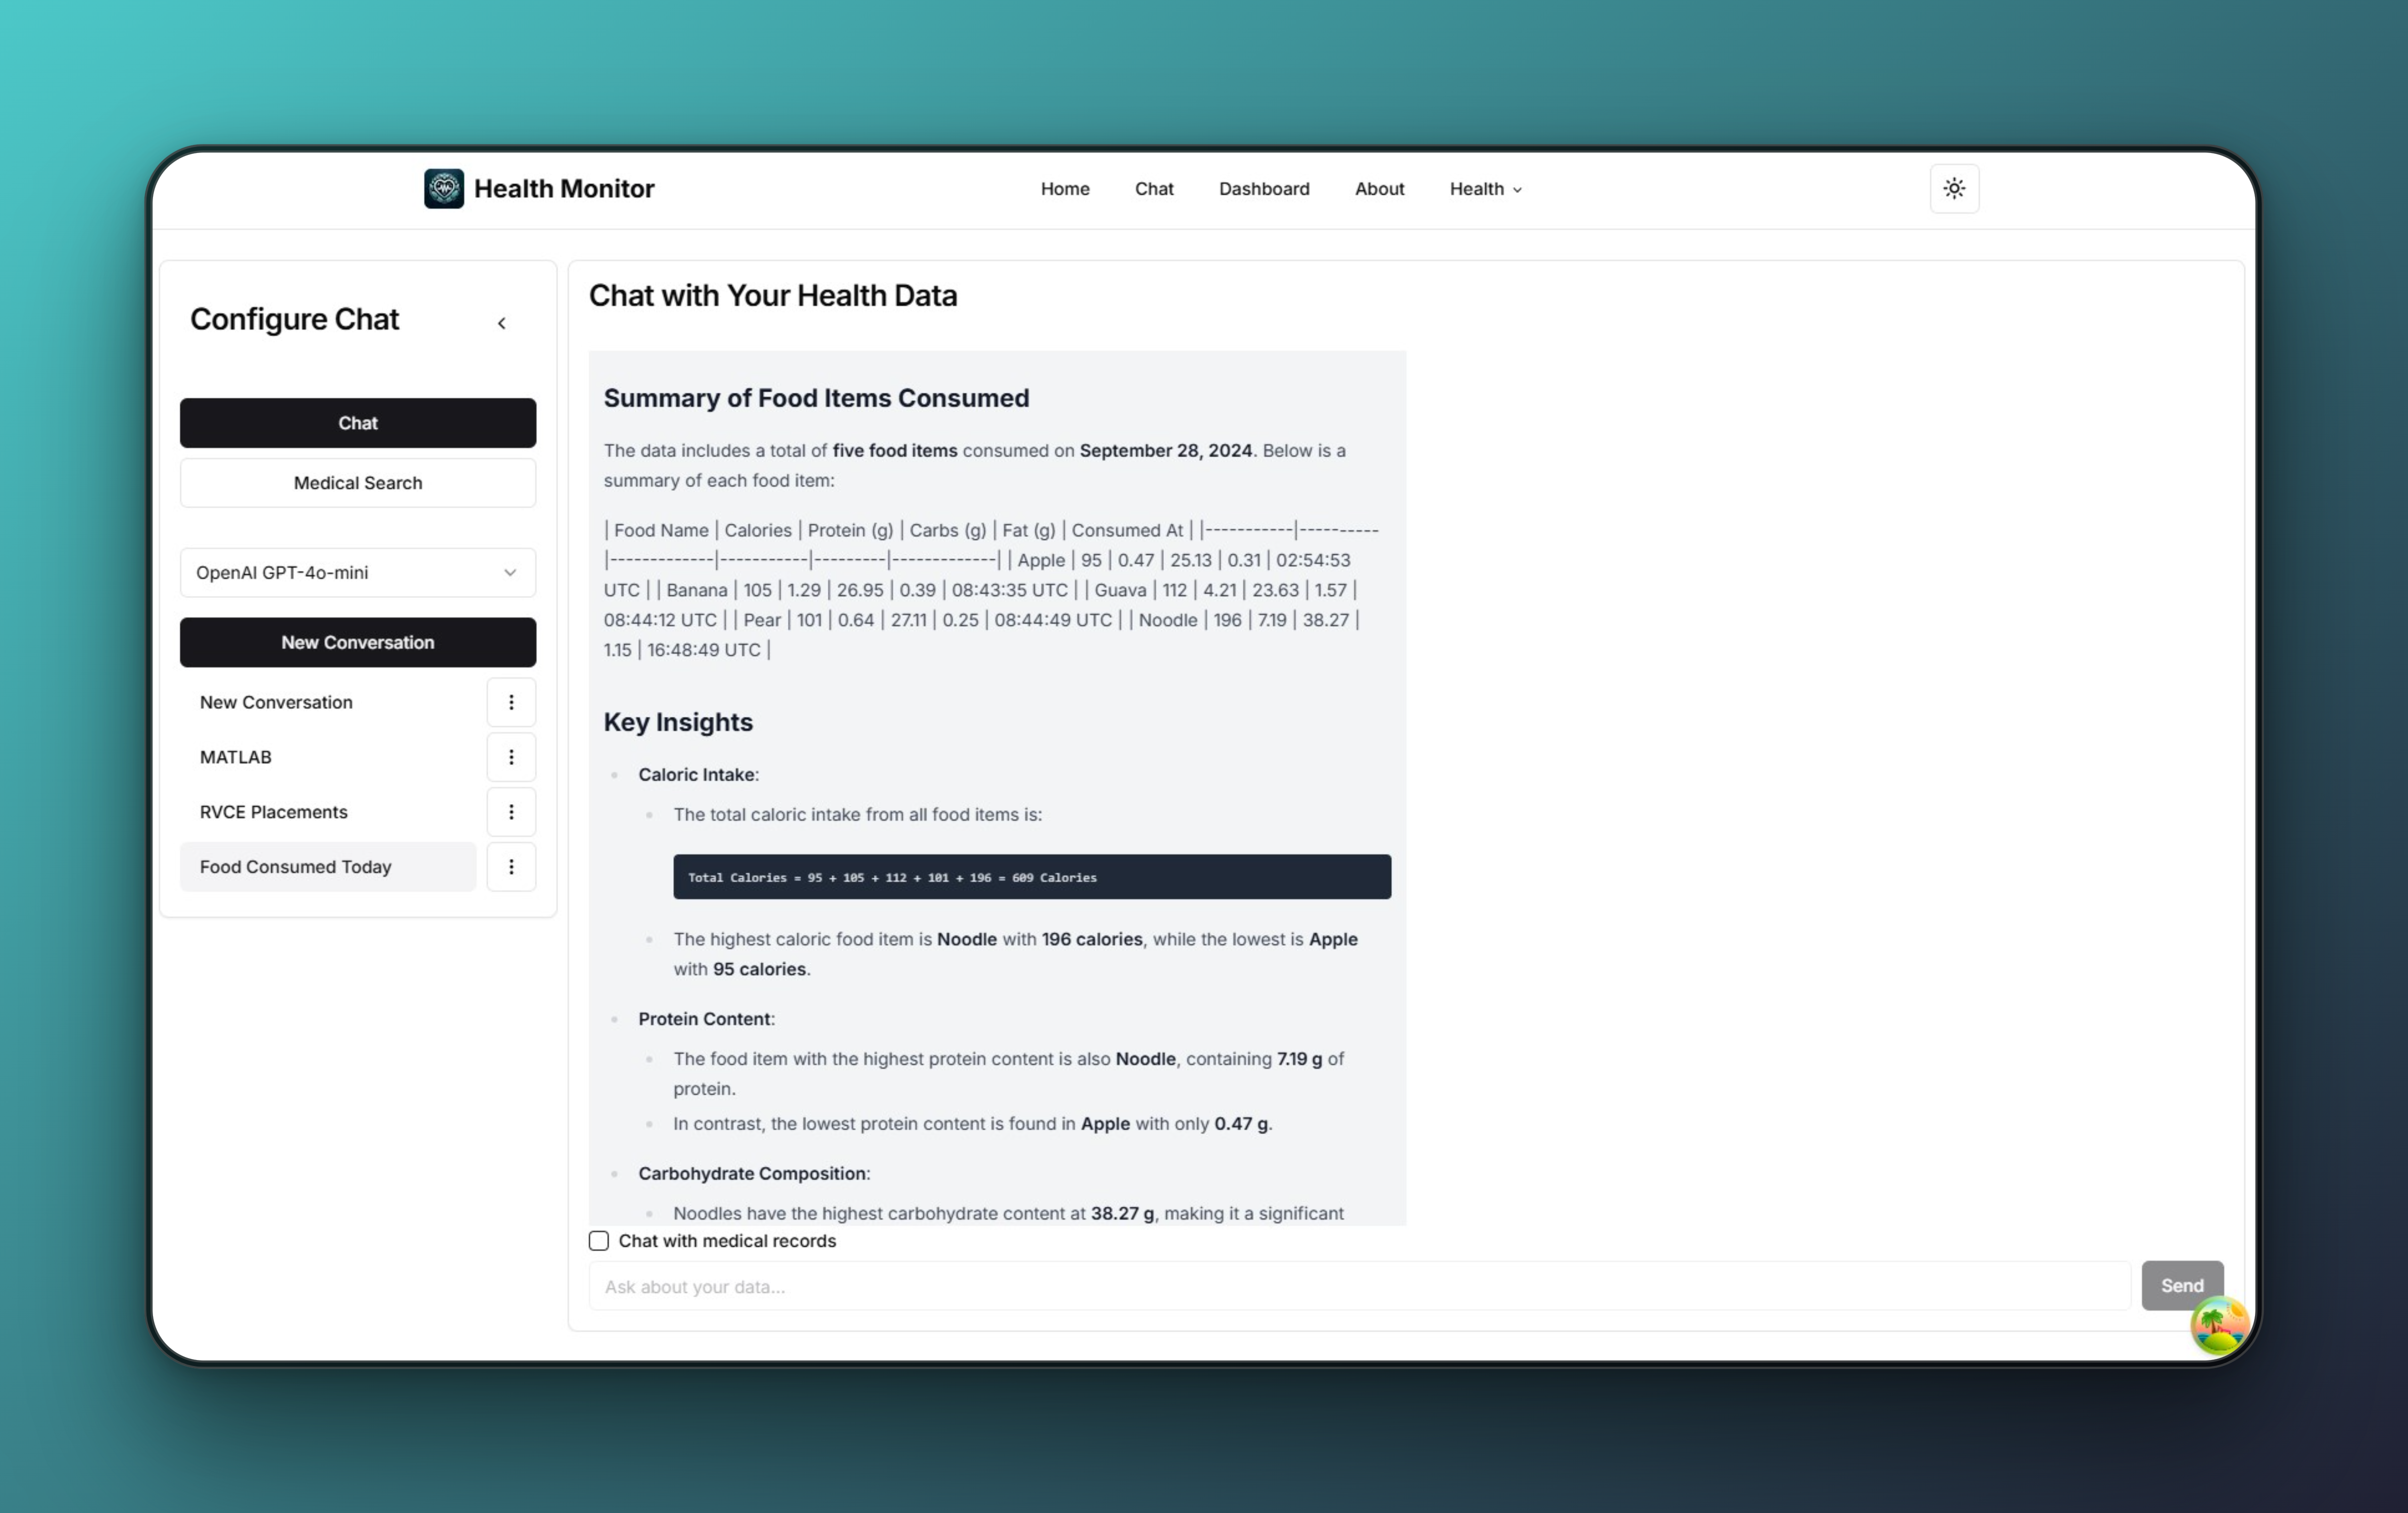
\includegraphics[width=0.8\textwidth]{public/landing/hm-chat-light.png}
    \caption{AI Health Assistant Interface}
\end{figure}

Implementation of AI features includes:
\begin{itemize}
    \item Natural language processing for user queries
    \item Context-aware response generation
    \item Medical terminology explanation
    \item Personalized health insights
\end{itemize}

\subsection{Data Visualization}
\begin{figure}[H]
    \centering
    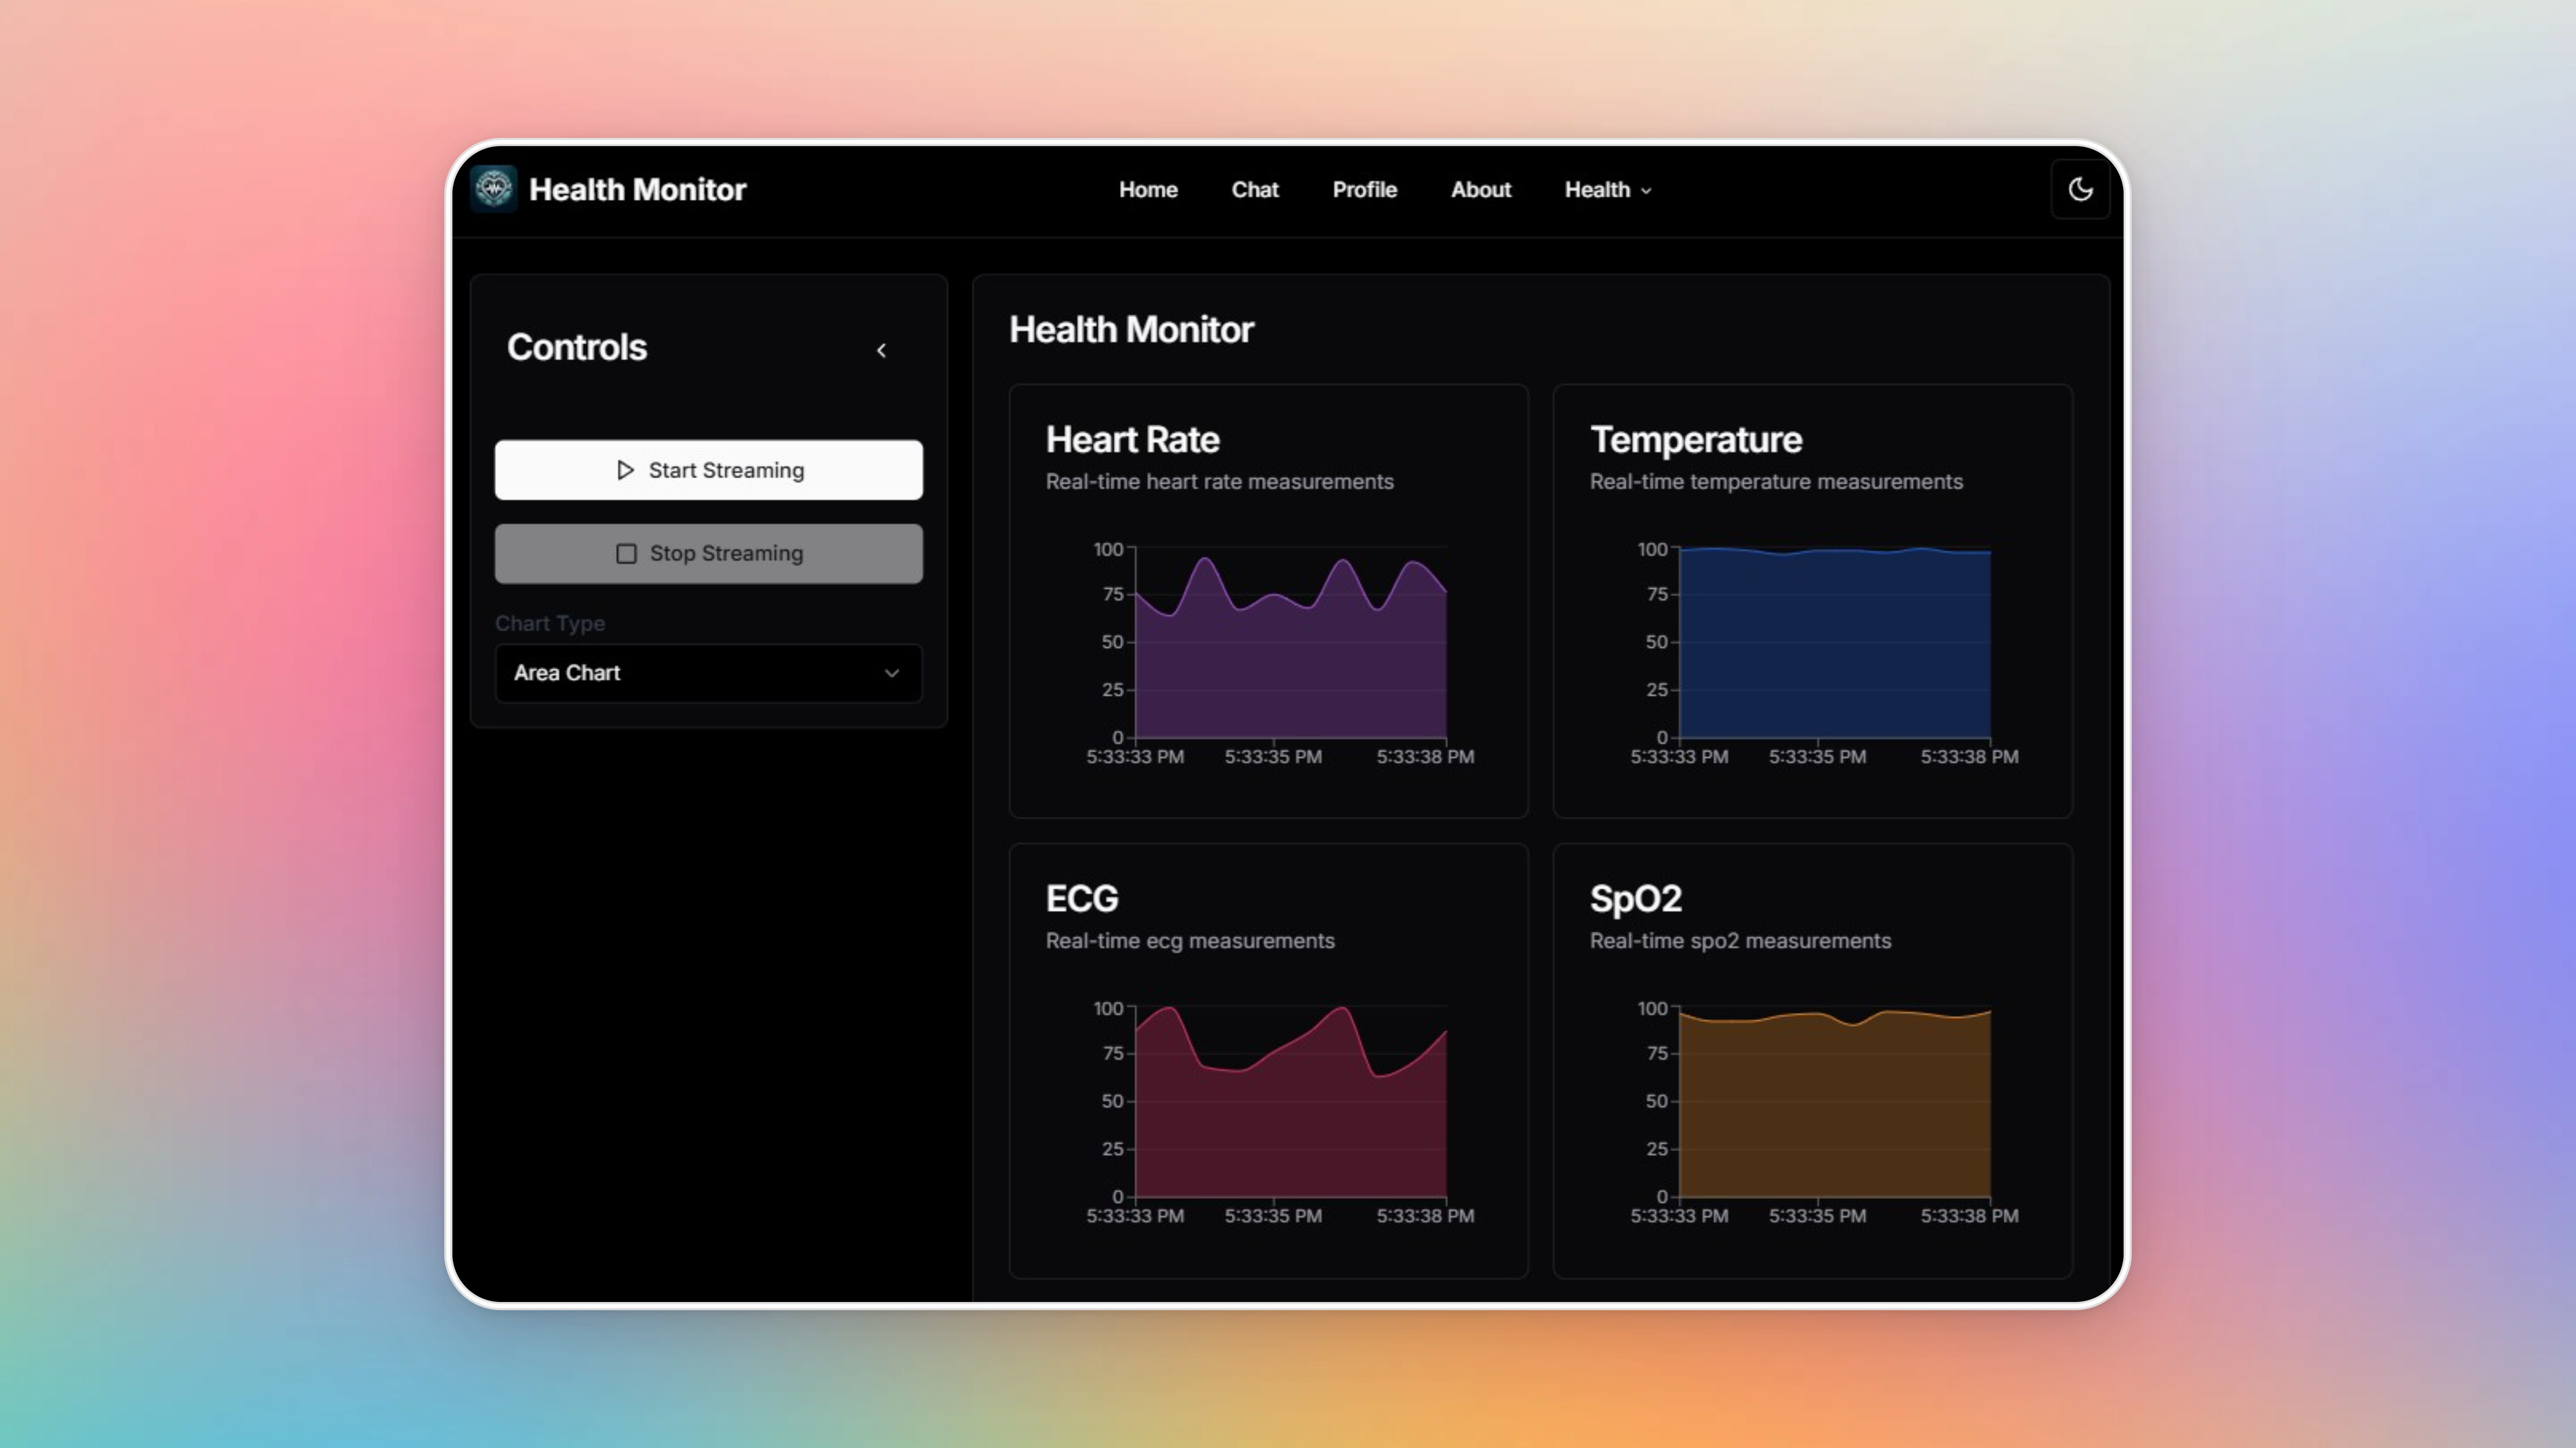
\includegraphics[width=0.8\textwidth]{public/landing/hm-graphs.png}
    \caption{Health Data Visualization Components}
\end{figure}

The visualization system includes:
\begin{itemize}
    \item Interactive charts and graphs
    \item Real-time sensor data display
    \item Health trend analysis
    \item Customizable dashboards
\end{itemize}

\subsection{Project Access}
The project can be accessed through:

\begin{itemize}
    \item GitHub Repository: \url{https://github.com/avinash-bharti/health-monitor}
    \item Live Demo: \url{https://health-monitor-demo.vercel.app}
    \item Documentation: Available in the repository's README
\end{itemize}

\section{Interface Screenshots}
The following screenshots showcase various aspects of the implemented prototype:

\subsection{Landing Page}
\begin{figure}[H]
    \centering
    \includegraphics[width=0.45\textwidth]{public/landing/hm-landing-new.png}
    \caption{HealthHub Main Landing Page}
\end{figure}

\subsection{Health Assistant Interface}
\begin{figure}[H]
    \centering
    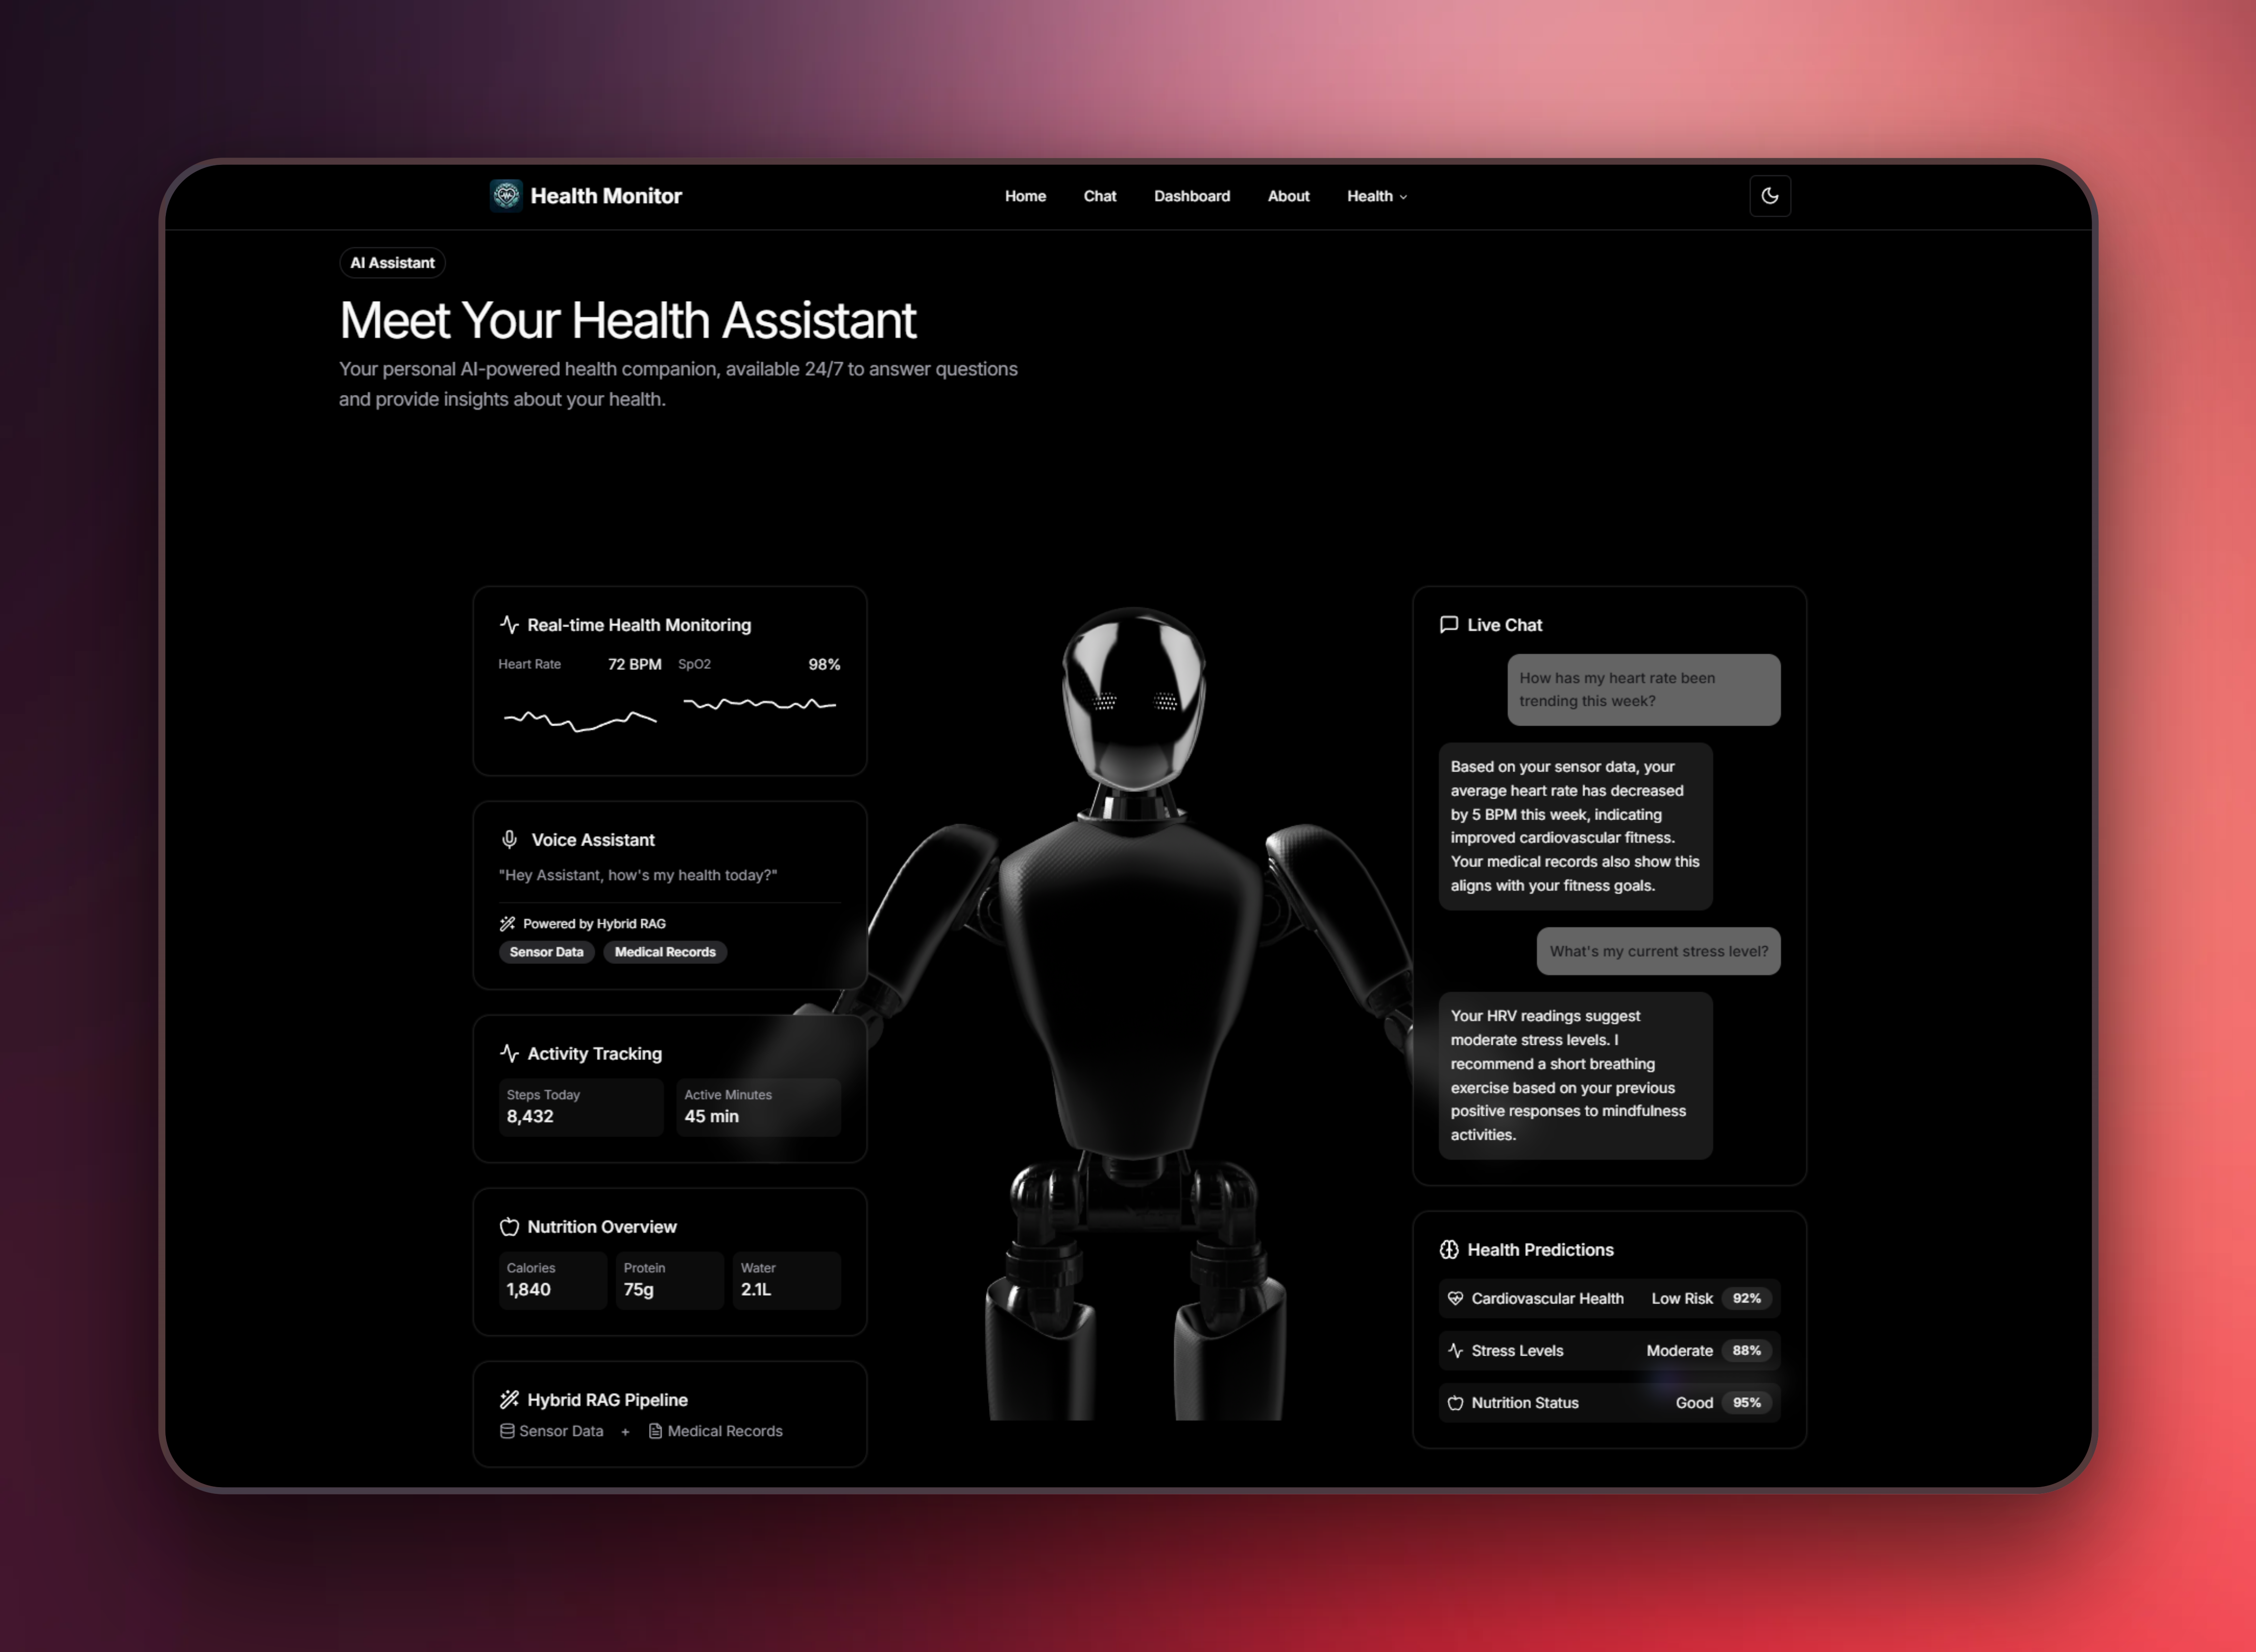
\includegraphics[width=0.45\textwidth]{public/landing/hm-landing-health-assistant-3.png}
    \caption{AI-Powered Health Assistant}
\end{figure}

\subsection{Dashboard and Analytics}
\begin{figure}[H]
    \centering
    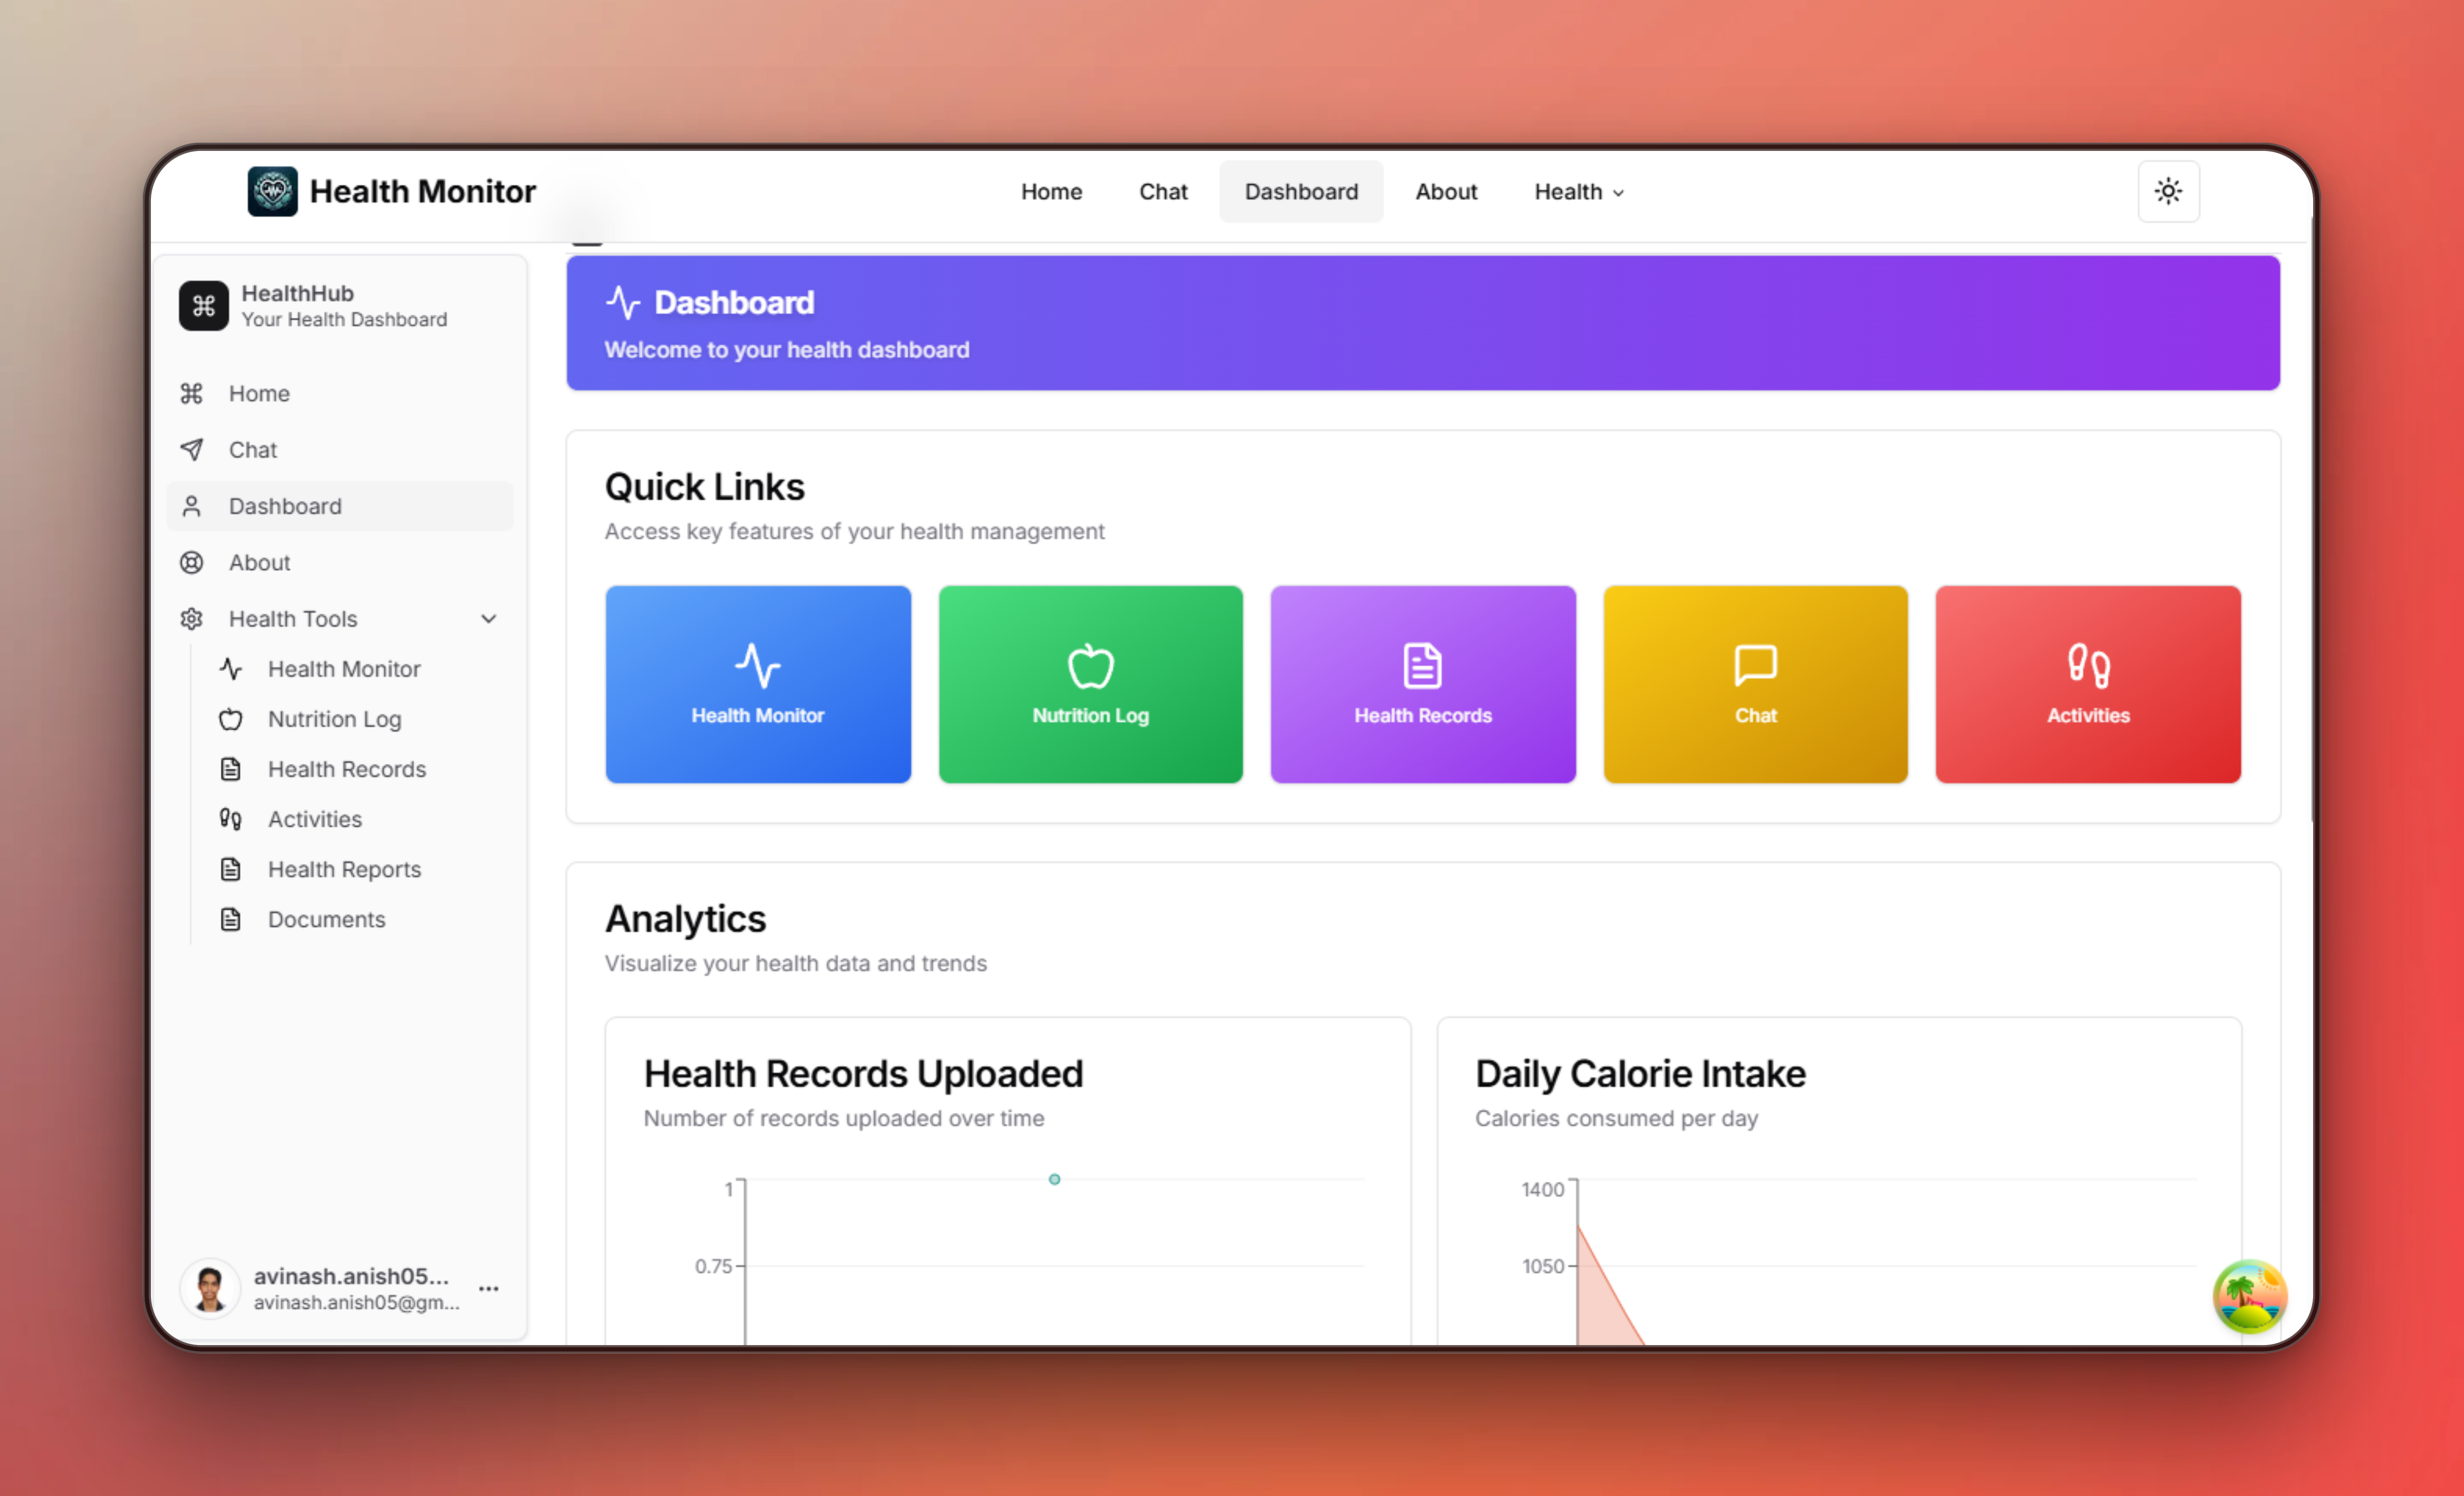
\includegraphics[width=0.45\textwidth]{public/landing/hm-dashboard.png}
    \caption{Interactive Dashboard Interface}
\end{figure}

\subsection{Data Visualization}
\begin{figure}[H]
    \centering
    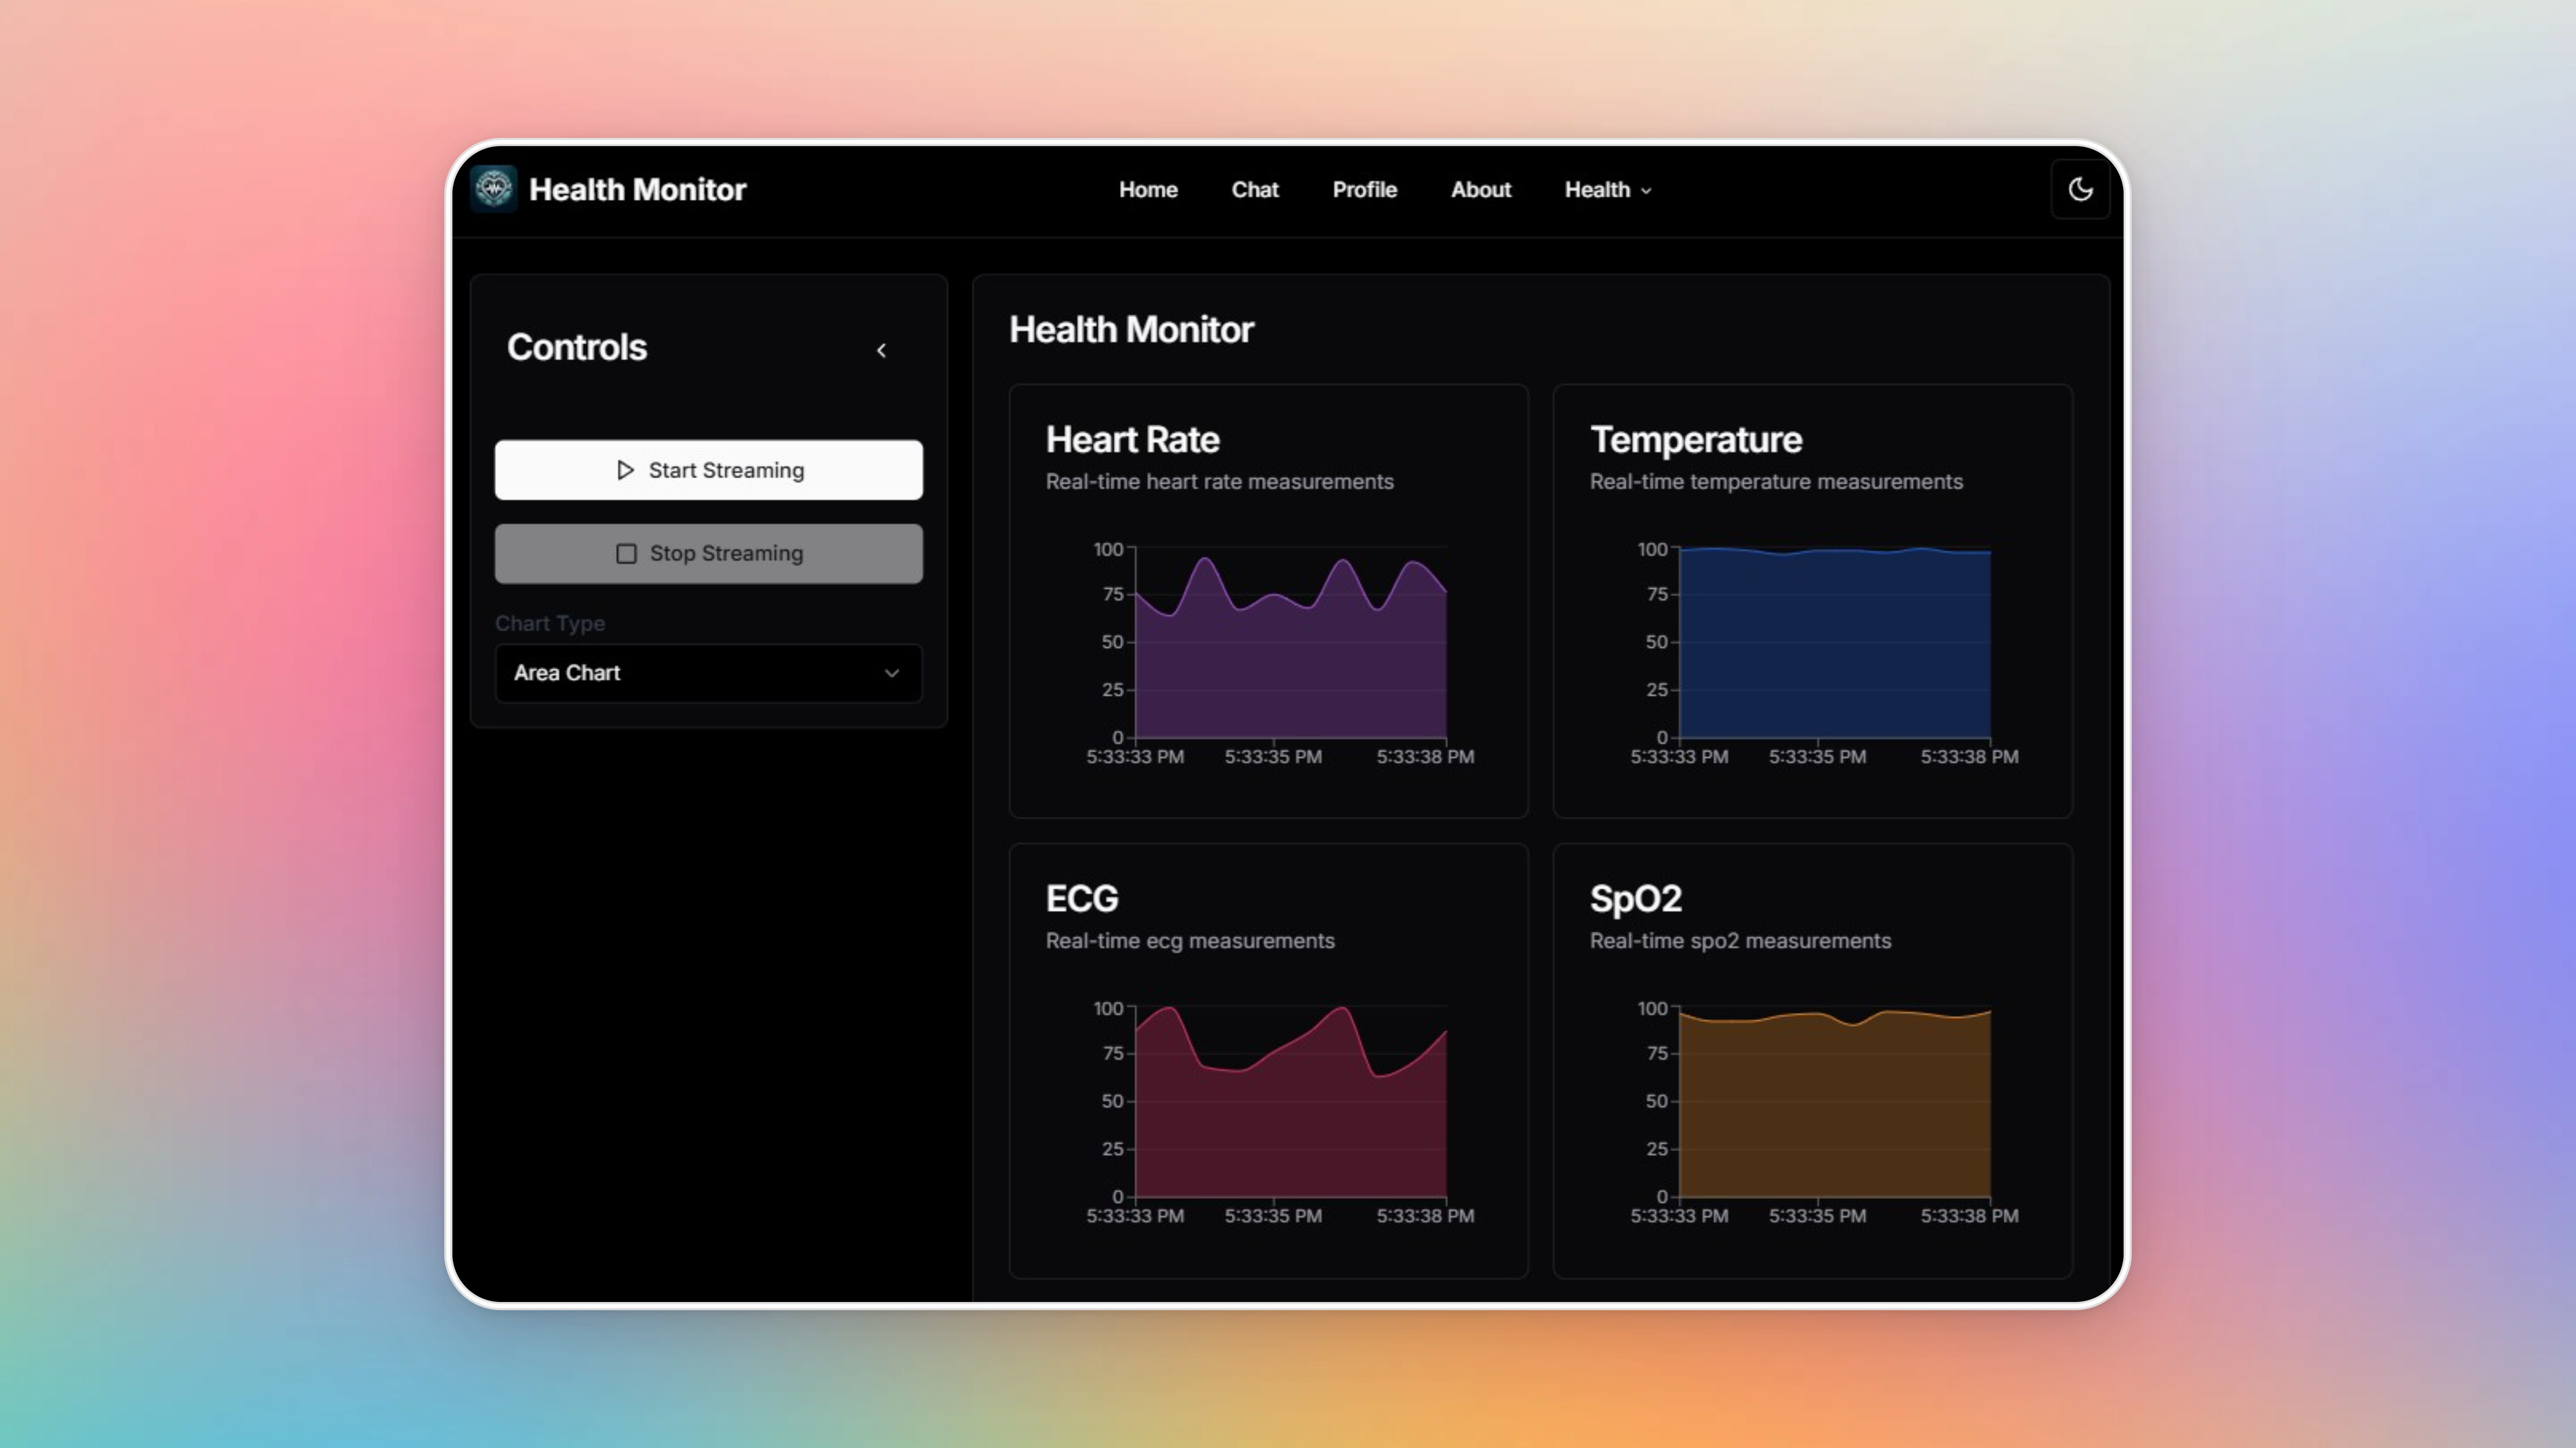
\includegraphics[width=0.45\textwidth]{public/landing/hm-graphs.png}
    \caption{Health Data Analytics and Visualization}
\end{figure}

\subsection{Record Management}
\begin{figure}[H]
    \centering
    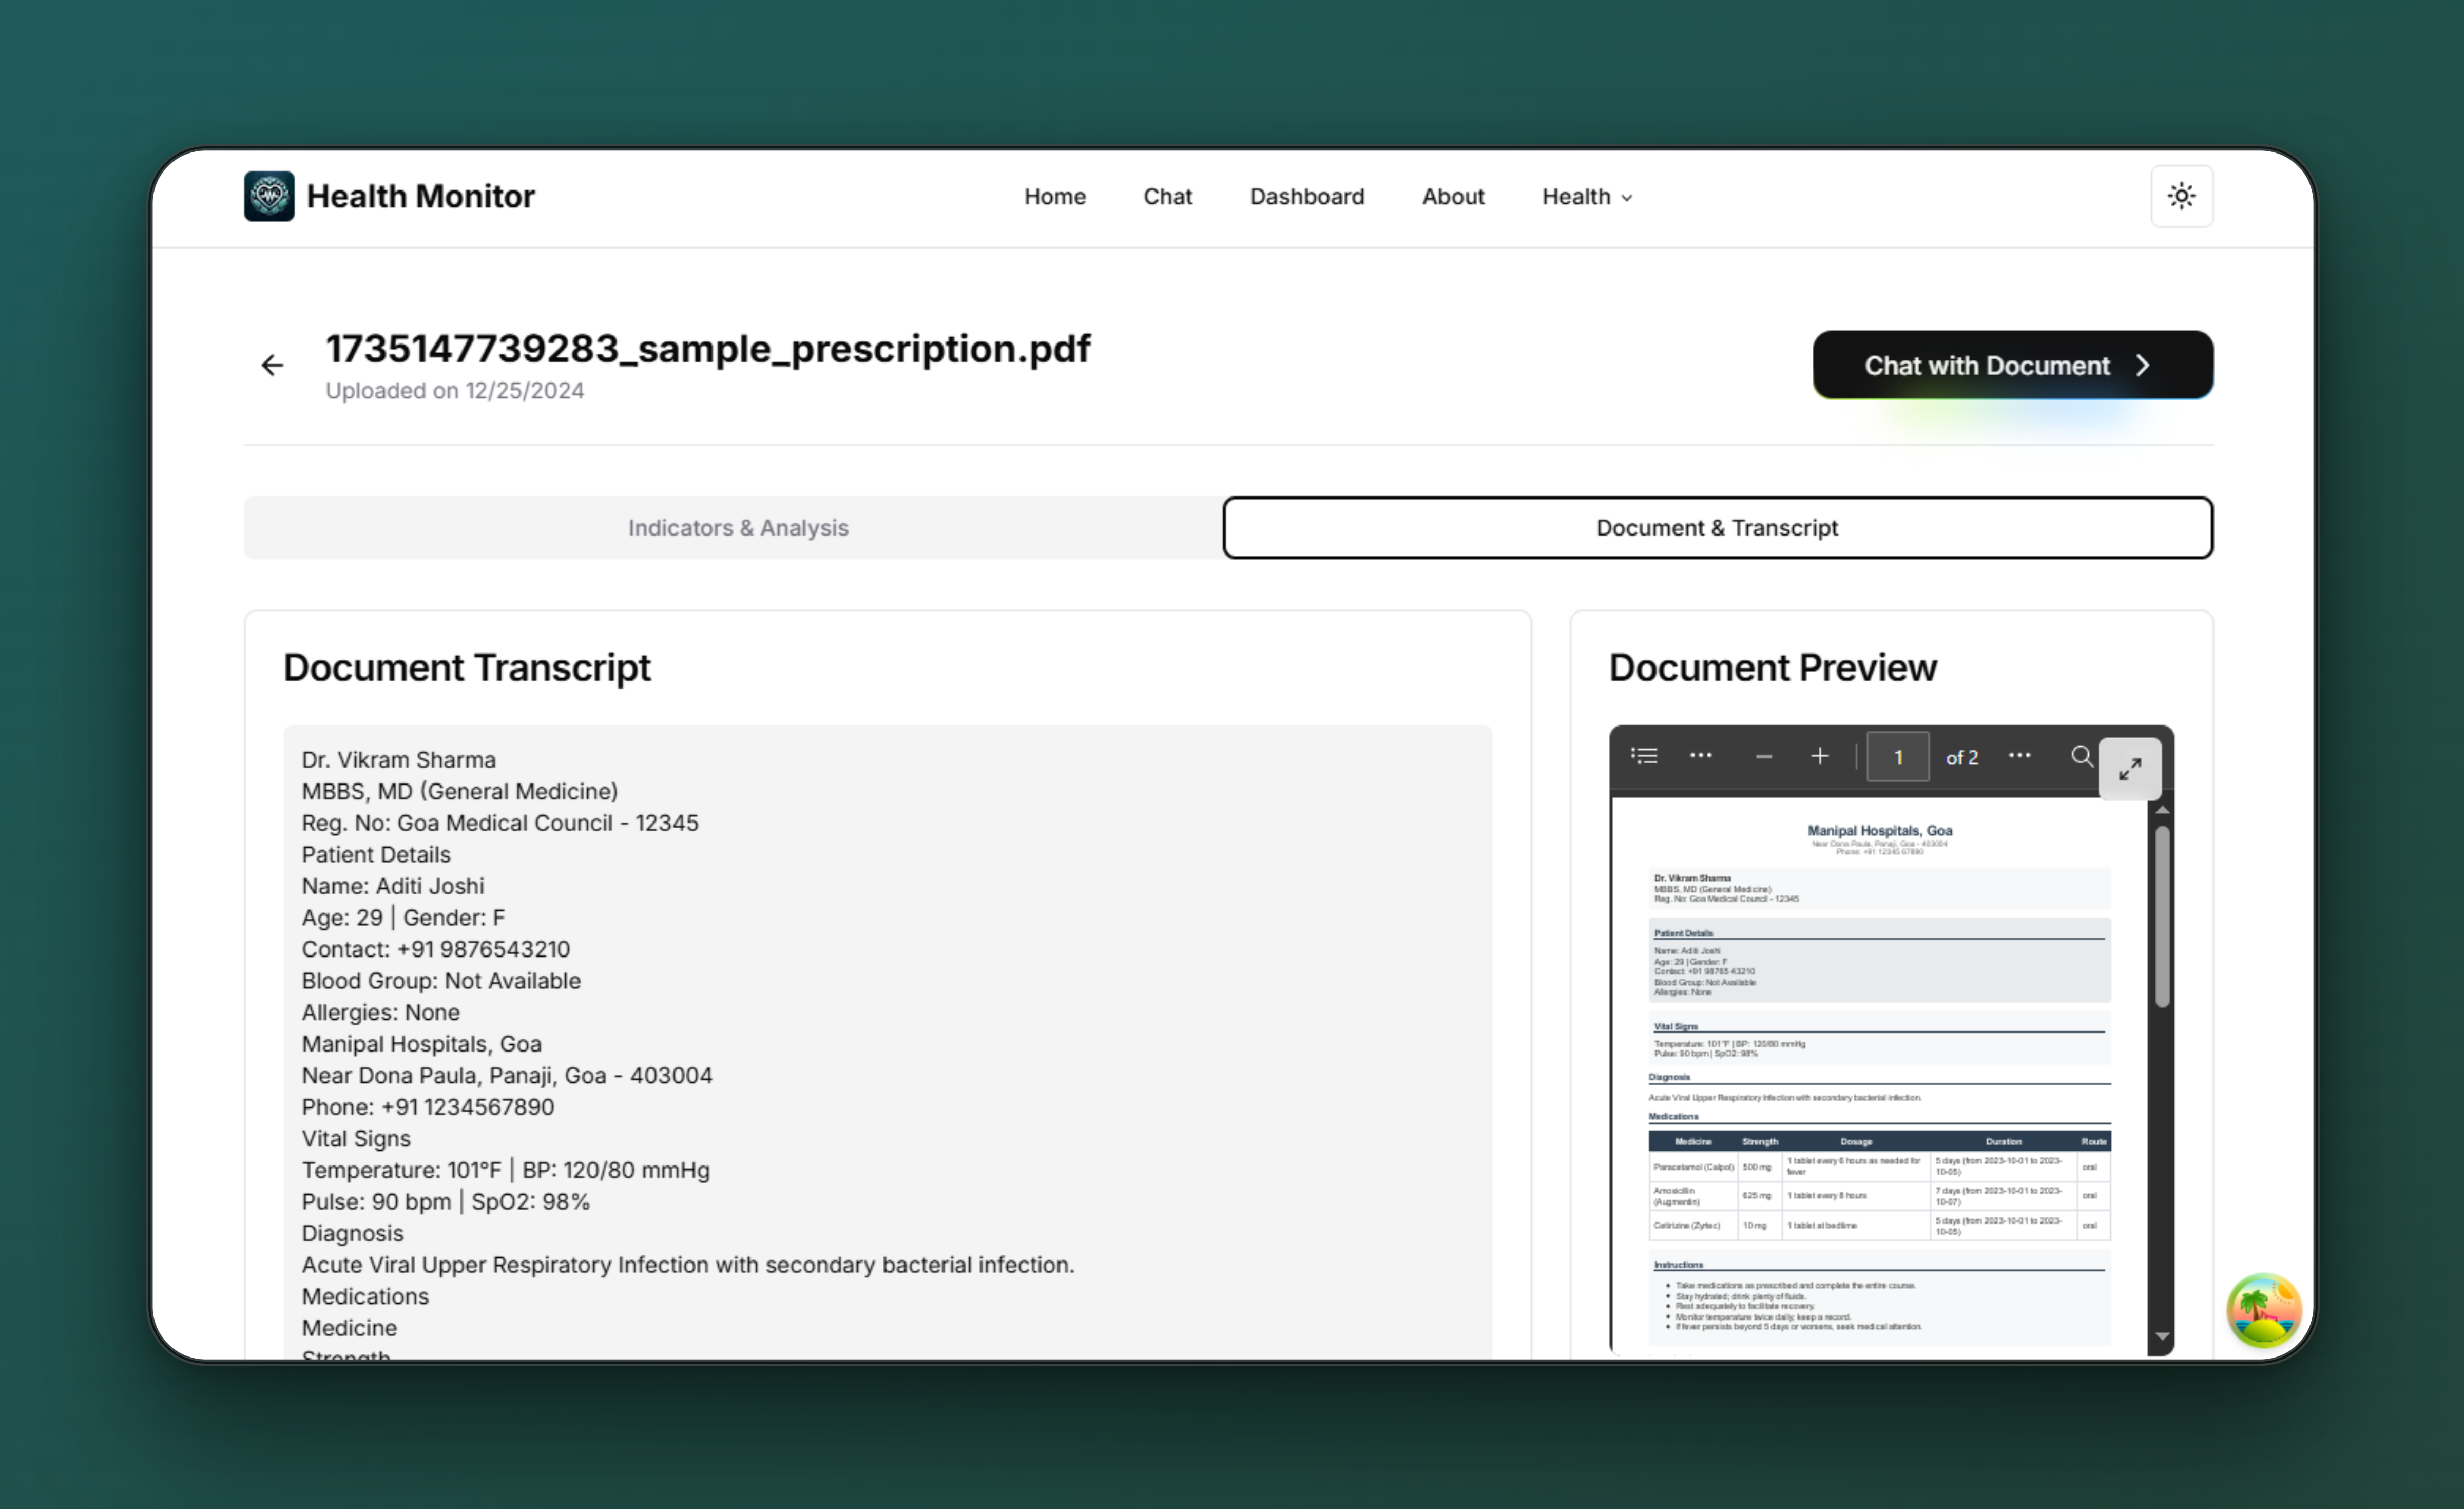
\includegraphics[width=0.45\textwidth]{public/landing/hm-record-transcript.png}
    \caption{Medical Record Processing Interface}
\end{figure}

\subsection{Analysis Reports}
\begin{figure}[H]
    \centering
    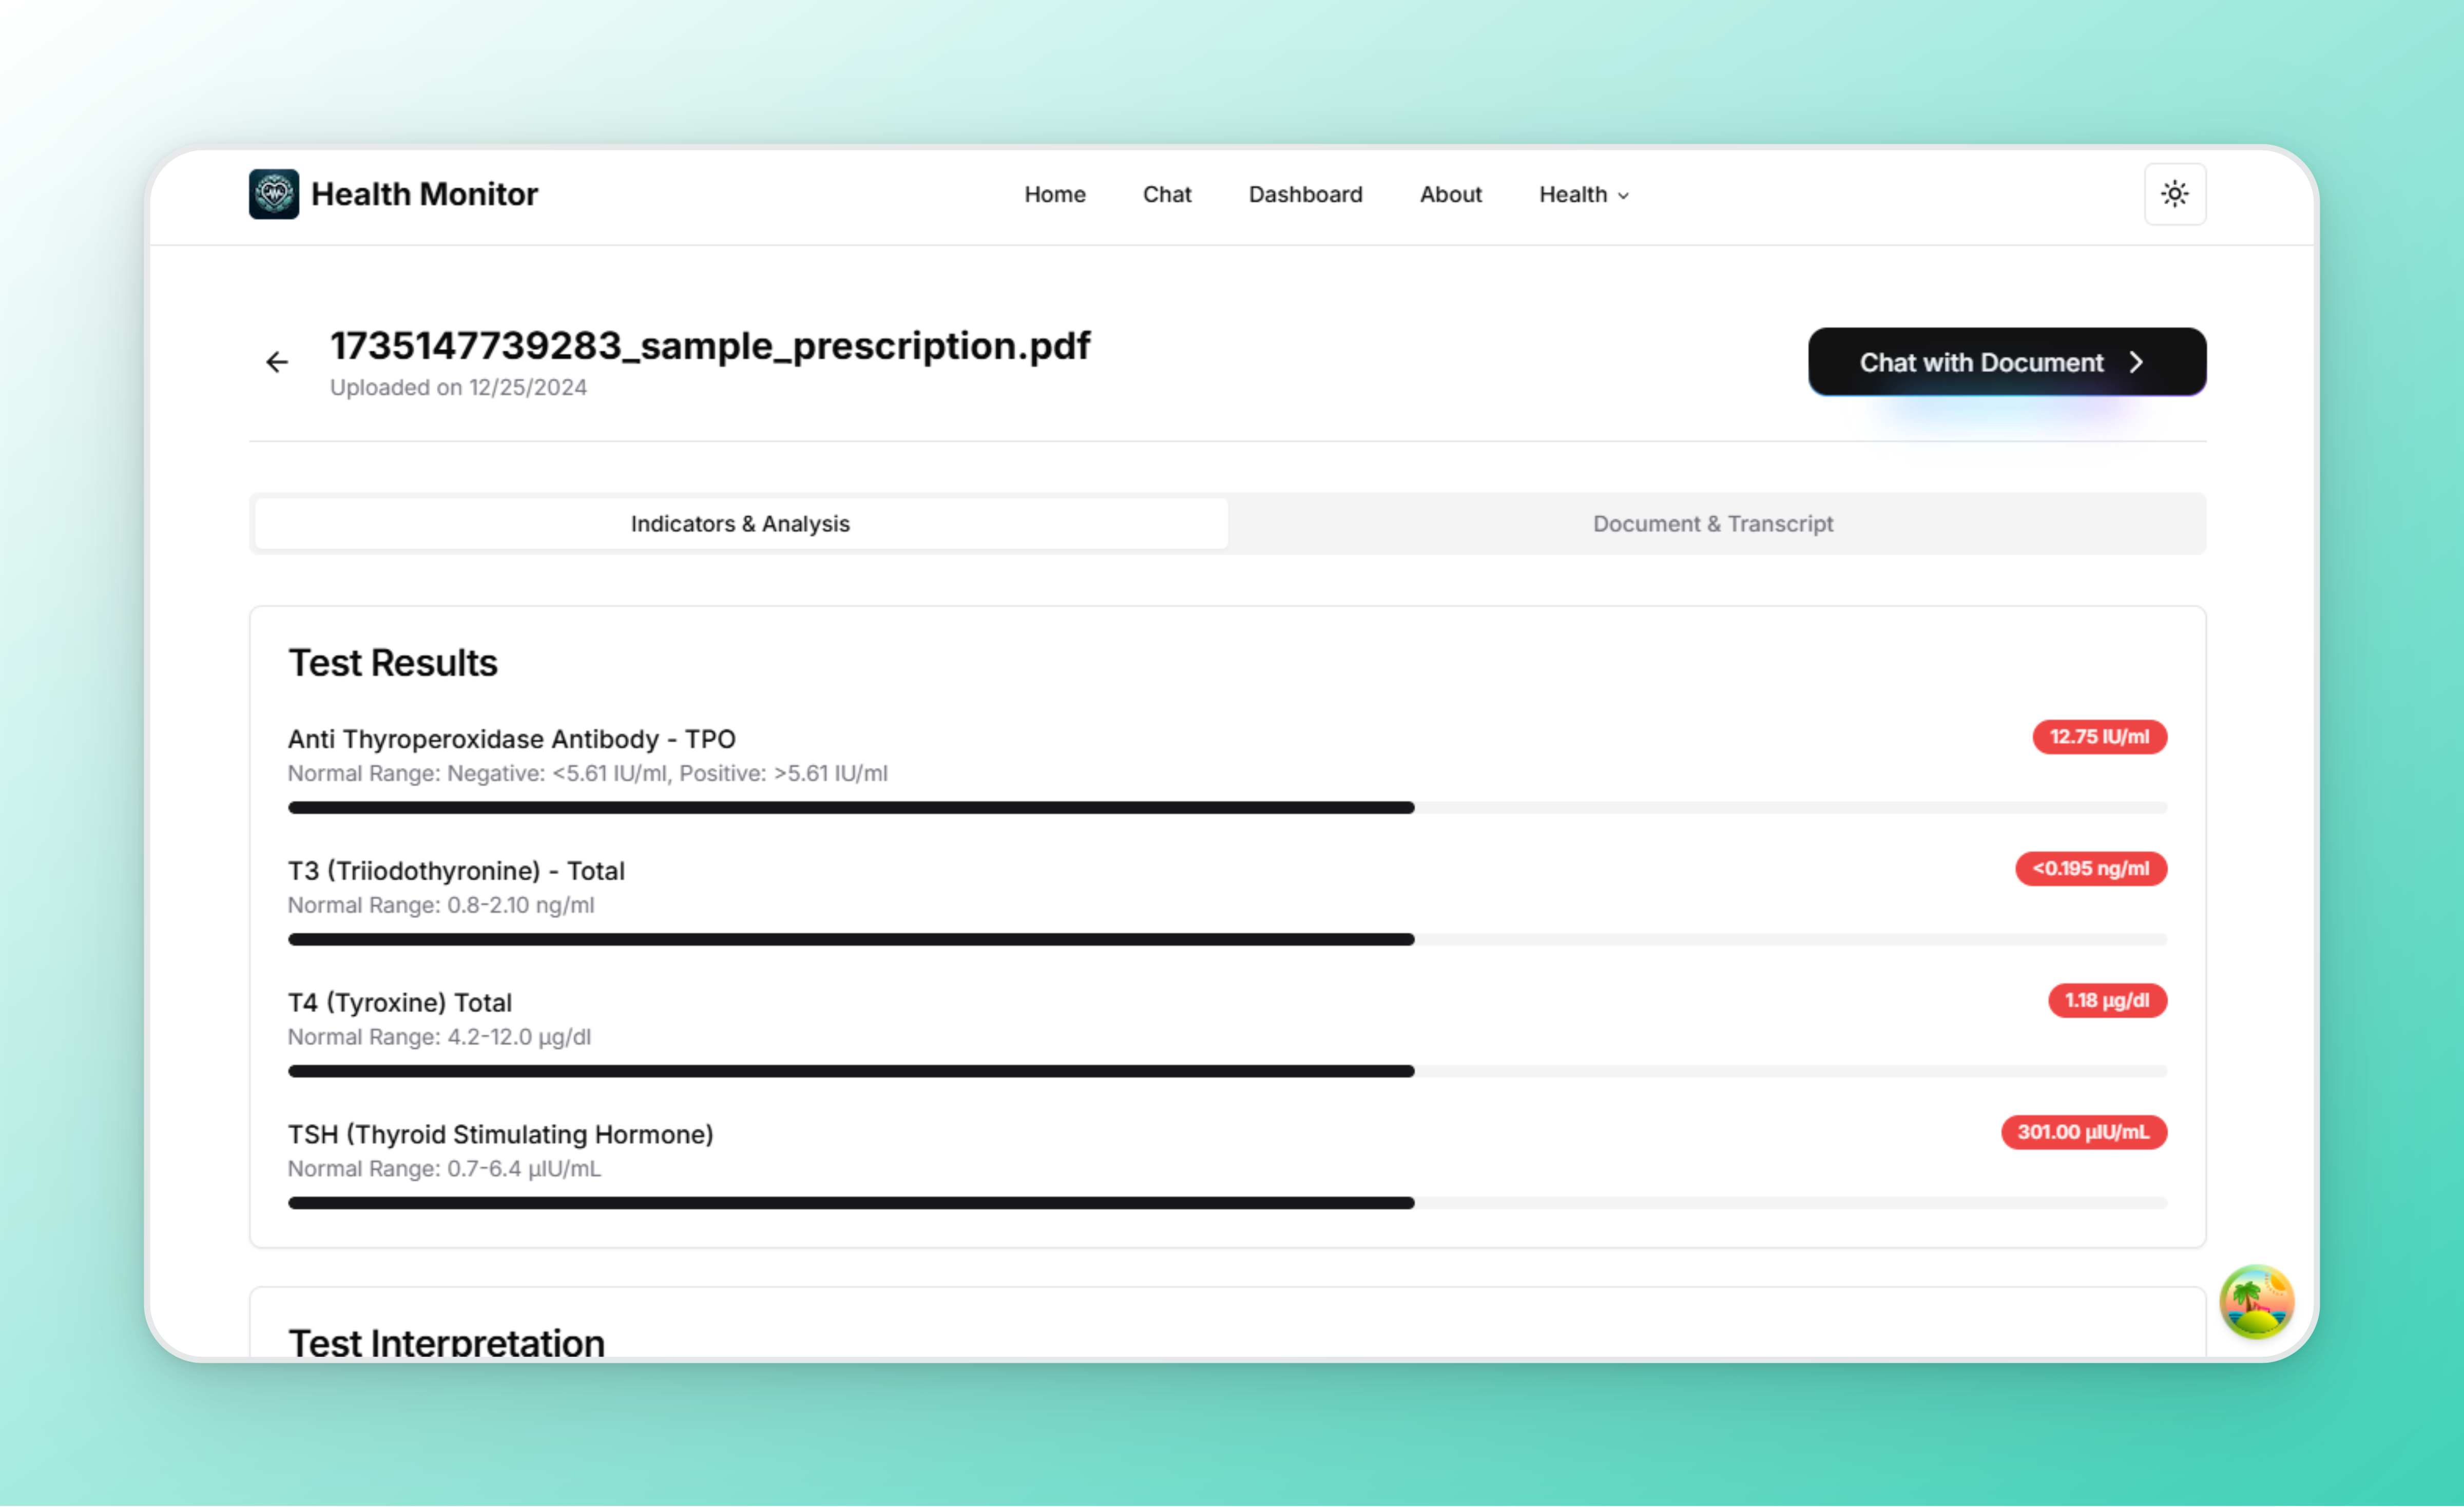
\includegraphics[width=0.45\textwidth]{public/landing/hm-record-analysis.png}
    \caption{Health Record Analysis View}
\end{figure}

\subsection{Activity Tracking}
\begin{figure}[H]
    \centering
    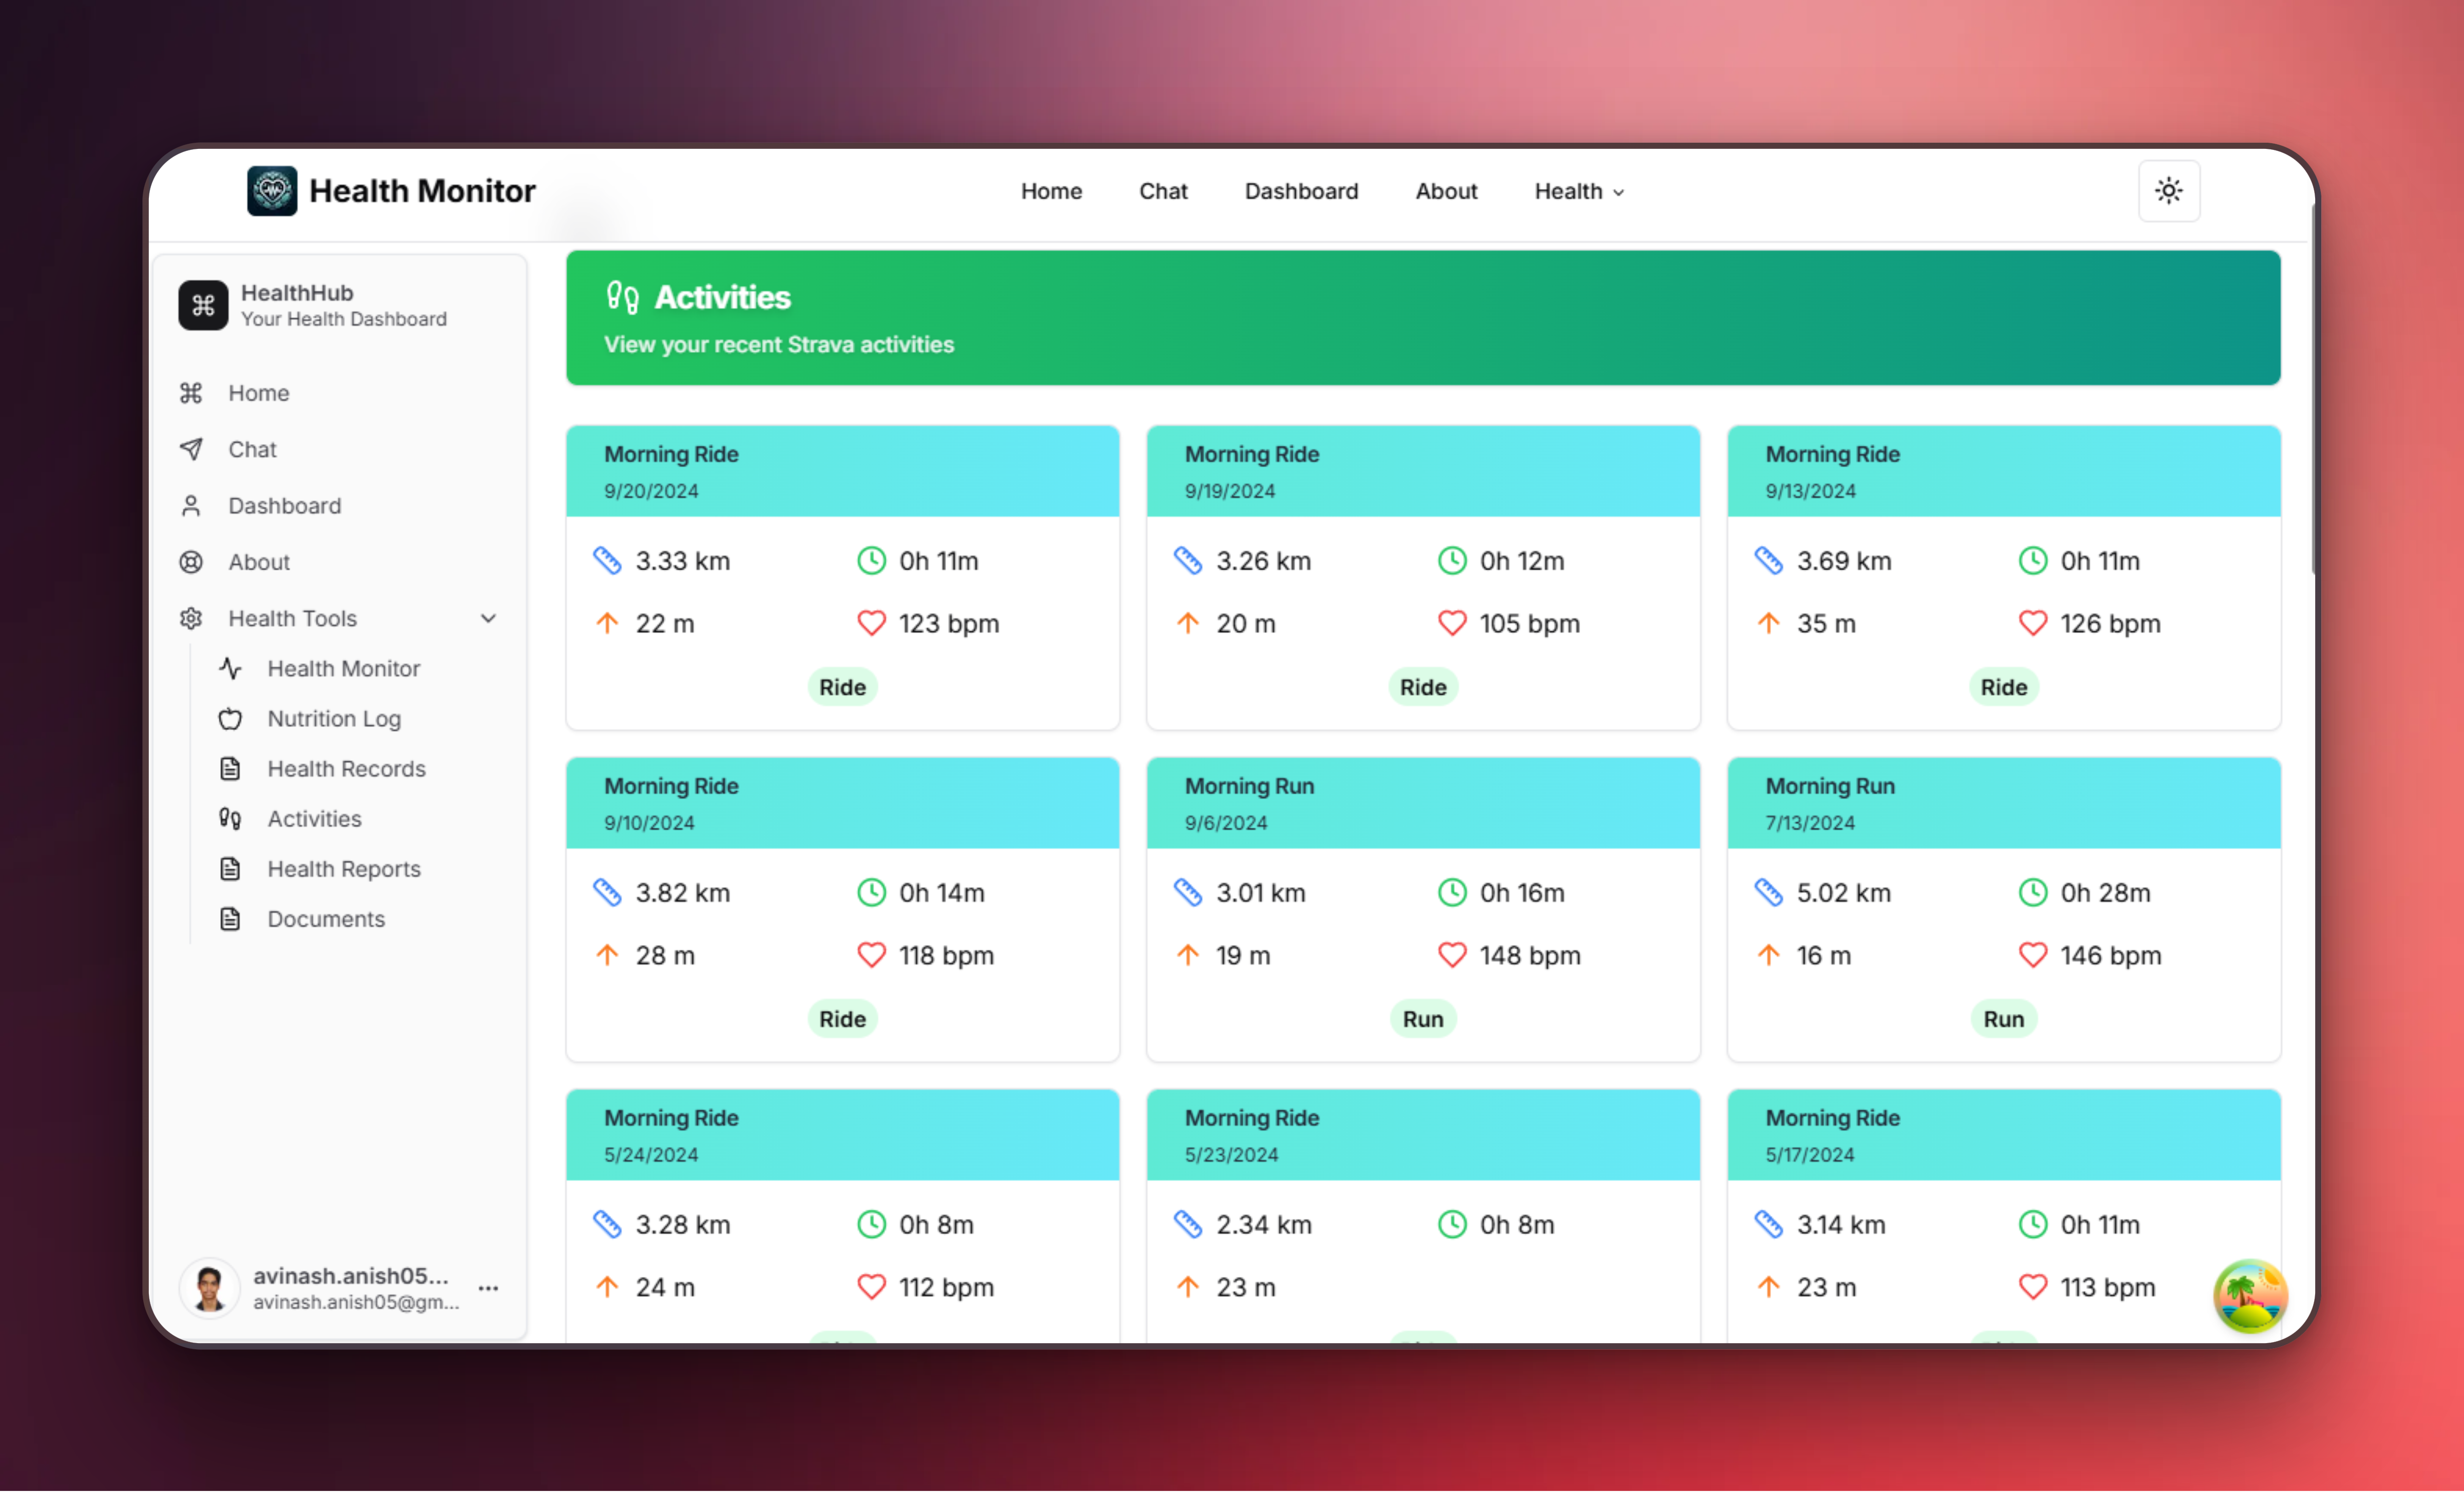
\includegraphics[width=0.45\textwidth]{public/landing/hm-activities.png}
    \caption{Physical Activity Monitoring Interface}
\end{figure}

\subsection{Nutrition Tracking}
\begin{figure}[H]
    \centering
    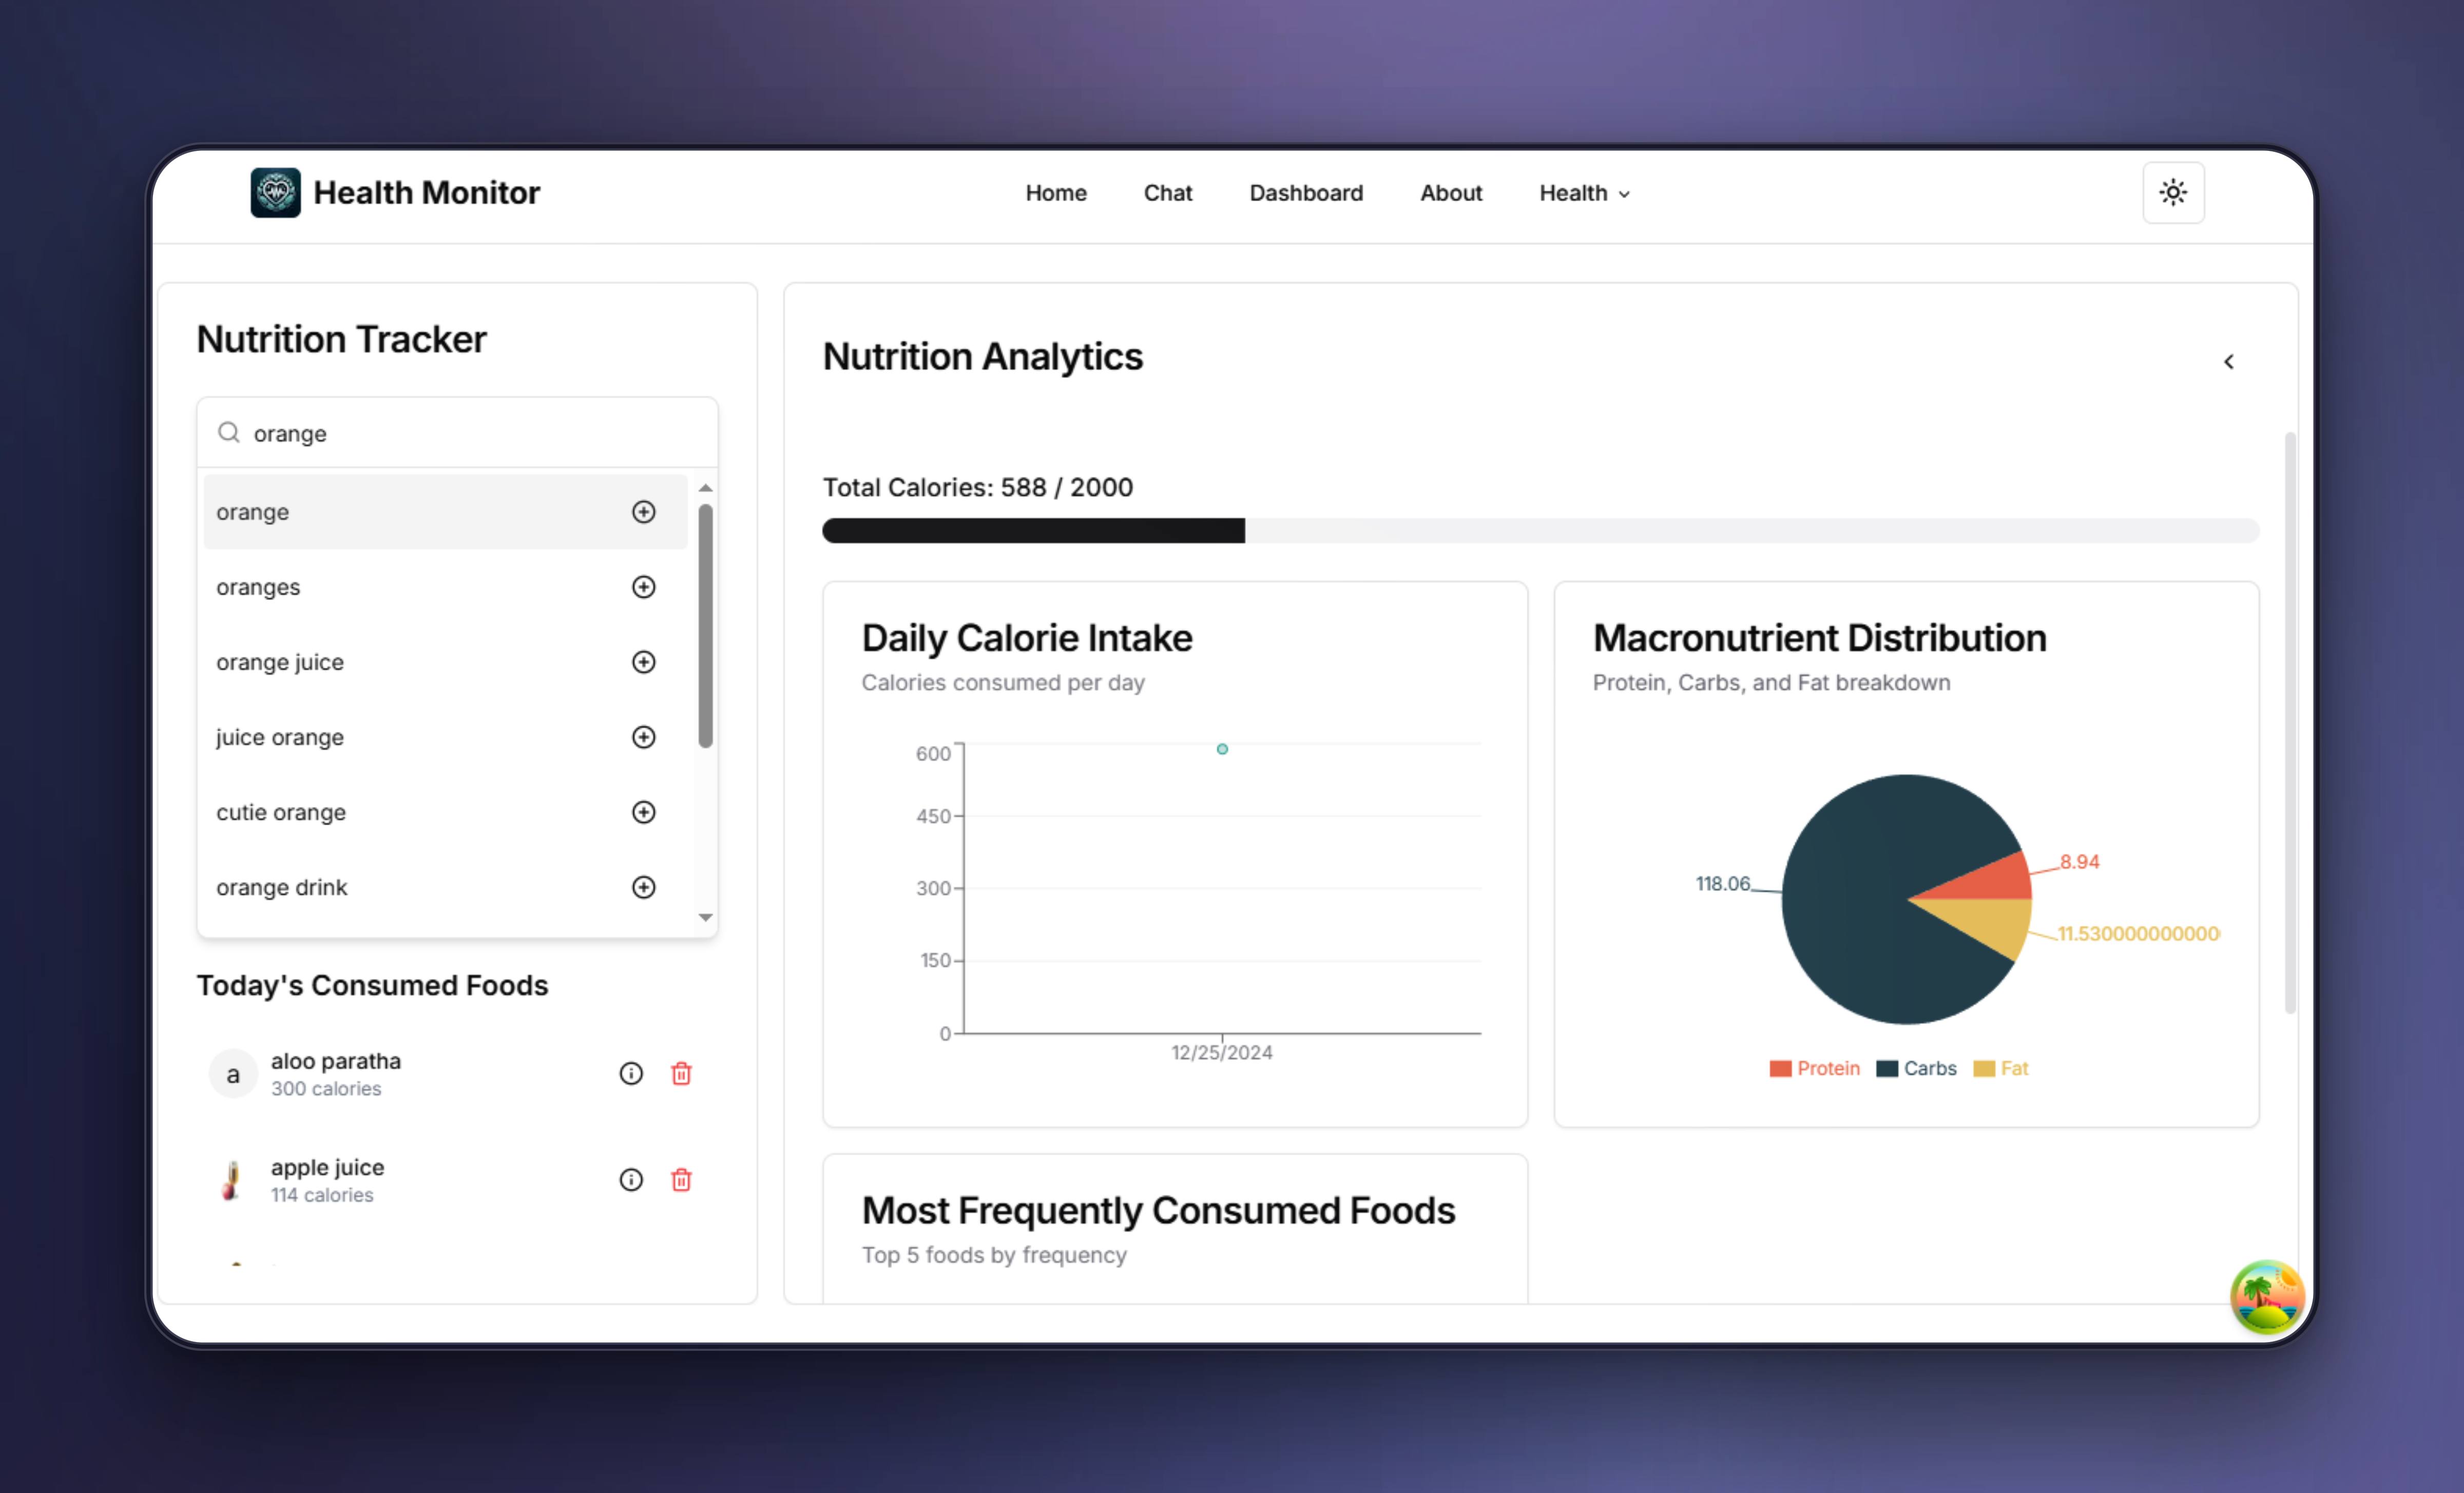
\includegraphics[width=0.45\textwidth]{public/landing/hm-nutrition.png}
    \caption{Nutrition Monitoring and Analysis}
\end{figure}

\section{Example Use Cases and Workflow}
\subsection{Example Queries and Responses}

To demonstrate the system's capabilities, here are some example interactions:

\begin{tcolorbox}[title=Query 1: Complex Medical History]
\textbf{User:} "What medications was I prescribed after my surgery last year, and how did they interact with my current heart condition?"

\textbf{System Response:}
\begin{itemize}
    \item Post-surgery medications: Tramadol (pain), Cephalexin (antibiotic)
    \item Current heart condition: Atrial fibrillation
    \item Interaction found: Tramadol noted to increase heart rate
    \item Recommendation: Switch to Acetaminophen
\end{itemize}

\textbf{Sources:}
\begin{itemize}
    \item Current heart rate: 72 bpm (sensor data)
    \item Surgical Report (07/15/2023)
    \item Cardiology Follow-up (08/02/2023)
\end{itemize}
\end{tcolorbox}

\begin{tcolorbox}[title=Query 2: Data Integration]
\textbf{User:} "How has my blood pressure changed since starting the new medication?"

\textbf{System Response:}
\begin{itemize}
    \item Pre-medication average: 145/90 mmHg
    \item Current average: 128/82 mmHg
    \item 12\% improvement in systolic pressure
    \item 720 sensor readings over 30 days
\end{itemize}
\end{tcolorbox}

\subsection{System Workflow}
The implementation follows a structured workflow for processing health data:

\subsubsection{Document Processing Pipeline}
\begin{enumerate}
    \item \textbf{Document Upload}
    \begin{itemize}
        \item User uploads medical records
        \item Frontend validates format and size
        \item Secure storage in Supabase
    \end{itemize}

    \item \textbf{Text Extraction}
    \begin{itemize}
        \item OCR processing using Tesseract
        \item Text cleaning and preprocessing
        \item Medical entity recognition
    \end{itemize}

    \item \textbf{Embedding Generation}
    \begin{itemize}
        \item Text chunking for processing
        \item Vector embedding via Cohere
        \item Storage in pgvector database
    \end{itemize}
\end{enumerate}

\subsubsection{Query Processing Flow}
\begin{enumerate}
    \item \textbf{Query Input}
    \begin{itemize}
        \item Natural language query reception
        \item Query embedding generation
        \item Context retrieval initiation
    \end{itemize}

    \item \textbf{Data Retrieval}
    \begin{itemize}
        \item Vector similarity search
        \item Real-time sensor data integration
        \item Structured data querying
    \end{itemize}

    \item \textbf{Response Generation}
    \begin{itemize}
        \item Context assembly
        \item LLM processing
        \item Response formatting and validation
    \end{itemize}
\end{enumerate}